\documentclass[12pt, a4paper, oneside]{book}
\usepackage{tfg}

% Notación
\renewcommand\nomgroup[1]{%
  \item[\bfseries%
  \ifstrequal{#1}{A}{Análisis}{%
  \ifstrequal{#1}{L}{Álgebra lineal}{%
  \ifstrequal{#1}{E}{Estadística}{%
  \ifstrequal{#1}{C}{Computación}{%
  }}}}%
]}
\renewcommand{\nompreamble}{En esta sección se describe el significado de los símbolos y la notación presente en este trabajo:}
\makenomenclature
\renewcommand{\nomname}{Notación}

% Bibliography
\addbibresource{references.bib}
\setlength{\abovedisplayskip}{3mm}
\setlength{\belowdisplayskip}{3mm}
\setlength{\abovedisplayshortskip}{0mm}
\setlength{\belowdisplayshortskip}{2mm}
%%%% Lengths

\pagestyle{plain}

\begin{document}
    \setcounter{page}{-1}
    \newpage
\thispagestyle{empty}

\begin{center}
    \rule{7cm}{1pt} \\
    \vspace*{0.2cm}
    \Large{Una introducción matemática a las redes neuronales} \\
    \large{Generative pre-trained transformers (GPT)}\\
    \rule{7cm}{1pt} \\
    \vspace*{1cm} 
    
\includegraphics[height=2in]{figures/escudo.jpg} \\
    \vspace{0.75cm}
    \Large{Trabajo de fin de grado} \\
    \Large{Curso 2022-2023} \\
    \vspace{0.5cm}
    \large{\textbf{Autor}} \\
    \large{Álvaro Sanz Ramos} \\ 
    \vspace{0.25cm}
    \large{\textbf{Director}} \\
    \large{Prof. Rosa María Pardo San Gil} \\

    \vspace{0.75cm}
    Doble grado en Ingeniería Informática y Matemáticas \\
    Facultad de Ciencias Matemáticas \\
    Universidad Complutense de Madrid \\
    \vspace{1cm}
\end{center}

    \newpage
    % \settowidth{\versewidth}{Ir y quedarse, y con quedar partirse}
\begin{verse}[\versewidth]
Ir y quedarse, y con quedar partirse, \\
partir sin alma y ir con alma ajena, \\
oír la dulce voz de una sirena \\
y no poder del árbol desasirse; \\[\baselineskip]

arder como la vela y consumirse \\
haciendo torres sobre tierna arena; \\
caer de un cielo, y ser demonio en pena, \\
y de serlo jamás arrepentirse; \\[\baselineskip]

hablar entre las mudas soledades, \\
pedir pues resta sobre fe paciencia, \\
y lo que es temporal llamar eterno; \\[\baselineskip]

creer sospechas y negar verdades, \\
es lo que llaman en el mundo ausencia, \\
fuego en el alma, y en la vida infierno. \\ 
\end{verse}
\attrib{Lope de Vega}

    \pagenumbering{roman}
    \setcounter{page}{1}
    \tableofcontents
    \printnomenclature[6em]

    \newpage
    \pagenumbering{arabic}
    \setcounter{page}{1}

    \cleardoublepage

\chapter{Introducción}
Posiblemente el lector ha interactuado con sistemas como Chat-GPT o Bard, asistentes capaces de conversar convincentemente sobre una variedad de temas, generar código o resolver exámenes. Estas herramientas tienen por núcleo redes neuronales profundas, llamadas \textit{grandes modelos de lenguaje}, diseñadas con una arquitectura concreta, la arquitectura \textit{transformer}, presentada por primera vez en 2017 \cite{vaswani2017attention}.

Desde su aparición, esta arquitectura se ha convertido en la opción preferencial para abordar problemas relacionados con el procesamiento de lenguaje natural, por su excelente rendimiento y por su notable escalabilidad, que permite construir modelos más grandes y potentes sin demasiados inconvenientes. 

Lo verdaderamente sorprendente es que, una vez que alcanzan una escala suficiente, los modelos basados en \textit{transformers} empiezan a mostrar \textit{habilidades emergentes}, volviéndose capaces de realizar tareas para las que no han sido entrenados \cite{wei2022emergent}. Los grandes modelos de lenguaje ya presentan un rendimiento mayor que los humanos en una multitud de tareas (por ejemplo, obtienen una calificación en el percentil 90 en el examen de acceso universitario en EEUU, SAT) y son considerados por algunos profesionales como el preámbulo de las inteligencias artificiales de propósito general \cite{bubeck2023sparks}.

Estos modelos no sólo tienen un interés teórico. Aunque el proceso de integración de los \textit{transformers} no ha hecho más que empezar, estos modelos ya se utilizan como traductores automáticos y asistentes conversacionales y se han integrado en los buscadores de Internet. Conforme se generalizan este tipo de redes, sus limitaciones se hacen más claras: pueden presentar de forma convincente resultados inventados (añadiendo citas y referencias inexistentes), ser engañados para desoír las indicaciones dadas por sus programadores o llegar a amenazar a los usuarios \cite{gpthallucination,gptthreats}. Su capacidad para ser confundidos con humanos, las convierte en temibles armas para la desinformación, la propaganda política o la publicidad. 

Existen, por tanto, razones más que sobradas para justificar el estudio de los \textit{transformers}: la elegancia de su diseño, lo amplio de sus posibilidades y  la urgente necesidad de comprender las amenazas y oportunidades que plantea su integración en nuestras sociedades.

\section{Objetivos del trabajo}
La velocidad de avance del campo del aprendizaje profundo y lo relativamente aislado de su comunidad, ha provocado un grave desfase entre la realidad del campo y los contenidos cubiertos por los manuales y otros recursos, la mayoría anteriores a la publicación de los \textit{transformers}.

Este trabajo se ha estructurado para ofrecer una introducción al campo del aprendizaje profundo y, específicamente, a las arquitecturas \textit{transformers} que requiere únicamente madurez matemática en los fundamentos de la teoría de la probabilidad, la inferencia estadística, el álgebra lineal y el cálculo multivariable, sin que sea necesario ningún conocimiento previo sobre redes neuronales.

El trabajo finaliza con una implementación del modelo GPT (probablemente la aplicación más influyente de la arquitectura \textit{transformer}) y su uso para abordar un problema complejo: crear una red neuronal capaz de generar texto al estilo de Lope de Vega. Por lo que sabemos, esta es la primera vez que se entrena una red similar para reproducir el estilo de un autor en lengua castellana. 

En conclusión, las metas fundamentales del trabajo son:
\begin{enumerate}[label=(O\arabic*)]
    \setlength{\itemsep}{0pt}
    \setlength{\parskip}{0pt}
    \item Presentar los conceptos generales sobre redes neuronales imprescindibles: qué es una red neuronal, qué propiedades tiene y cómo puede entrenarse.
    \item Presentar el problema de procesamiento de lenguaje natural y sus singularidades. Realizar una revisión del estado de la cuestión.
    \item Presentar la arquitectura \textit{transformer} y ponerla en relación con arquitecturas anteriores. Entender cómo puede modificarse para abordar problemas diversos, como la generación de texto
    \item Implementar \textit{GPT} y utilizar la arquitectura para abordar el problema de generar texto en el estilo de Lope de Vega. Evaluar el rendimiento y discutir alternativas y limitaciones.
\end{enumerate}

\section{Plan de trabajo}
La adquisición de los rudimentos del campo del aprendizaje automático se ha realizado en colaboración con varios compañeros, bajo la supervisión de la directora del trabajo, la profesora Pardo San Gil. 

A partir de estas bases, se ha profundizado, mediante el estudio autónomo, en el campo de las arquitecturas \textit{transformer}. La gran mayoría de la literatura no tiene como prioridad la formalización matemática de los conceptos introducidos, con lo que ha sido necesario encontrar abstracciones adecuadas que permitan su discusión inequívoca.

Una vez sentada la base teórica, y en paralelo a la creación de esta memoria, se ha implementado la arquitectura y aplicado al problema propuesto. Esta tarea requiere familiaridad con las librerías de programación contemporáneas, obras de ingeniería de gran complejidad.

Finalmente, tanto los resultados teóricos como las aplicaciones prácticas que se recogen en esta memoria han sido presentadas al grupo de estudio inicial, en dos presentaciones de 50 y 10 minutos respectivamente, bajo la supervisión de la profesora Pardo San Gil. Dichas presentaciones, así como la revisión llevada a cabo por la directora, se han probado de gran utilidad para dar su forma final a este trabajo.




    \chapter{Redes neuronales pre-alimentadas}
Realizamos en este capítulo una breve introducción a las redes neuronales secuenciales, inspirada en algunos de los más influyentes manuales sobre el tema \cite{goodfellow2016deep, bishop2006pattern}.

Es habitual presentar las redes neuronales de ``abajo a arriba'', comenzando por el concepto de \textit{neurona artificial} y definiendo las redes neuronales como conjuntos de neuronas conectadas. Este enfoque, el más fiel al desarrollo histórico, omite el hecho de que las redes neuronales contemporáneas no están compuestas íntegramente por neuronas, sino que presentan componentes de naturaleza y propósito muy distinta, como la normalización y regularización. 

En este capítulo se realiza una presentación alternativa de las redes neuronales, centrada en el concepto de capa, se estudian sus propiedades teóricas y se introducen los problemas de diseño y entrenamiento de las redes neuronales.

\section{Conceptos básicos}
Dado un espacio de entrada \( X \subset \real{n} \) y un espacio de salida \( \real{m} \), una red neuronal es un modelo matemático que computa una función \( f: X \to \real{m} \) definida de forma composicional mediante una sucesión de \textit{capas} \( \Set{l_{i}}_{i=1}^n \), cada una de las cuales calcula una función \( f_{i} \). Por lo general, \( f_{i} \) es una función parametrizada (es decir, \( f_{i} = f_{i}(\mathord{\smallbullet}; \theta_i) \)); siendo \( \theta = \Set{\theta_i \mid i = 0 … n} \) el conjunto de parámetros del modelo.

Las capas están \textit{enlazadas} entre sí, de forma que la salida de una capa proporciona la entrada a otras capas. Podemos definir una red neuronal mediante la tupla \( (X, \real{m}, \Set{ l_i }, \Sigma) \), siendo \( \Sigma \) una especificación de las conexiones entre capas.

En principio, las conexiones entre capas pueden ser muy complejas: por ejemplo, no es infrecuente que la entrada de una capa provenga de concatenar la salida de varias capas. Las redes neuronales más sencillas son las \textit{secuenciales}, aquellas en las que la salida de una capa es la entrada de la siguiente, de forma que \( f = f_{0} \cdot f_{1} \cdot … \cdot f_{n} \).

Una forma más debil de la \textit{secuencialidad} es la \textit{retroalimentación}: una red es retroalimentada si no existen ciclos en los enlaces entre capas. En este caso, la capa \( l_0 \), que recibe los datos proporcionados a la red neuronal, se denomina la \textit{capa de entrada}, la capa \( l_{n} \) es la \textit{capa de salida} y el resto de capas se denominan \textit{capas ocultas}.

Este trabajo se centra en el estudio de las redes retroalimentadas, dado que las redes no retroalimentadas (\textit{recurrentes}) presentan sus problemas propios.

Durante mucho tiempo, el concepto de red neurronal fue sinónimo de \textit{perceptrón multicapa}, una red secuencial en la que todas las capas son \textit{capas de neuronas}:
\begin{definition}[Capa de neuronas]
    Dada una matriz \( W \in \real{m \times n} \), un vector \( b \in \real{m} \) y una función \( \sigma: \realo \to \realo \) una capa de neuronas computa una función \( \MLP: \real{n} \to \real{m} \)
    \[
        \MLP(x; W, b) = \sigma(Wx + b)
    \]
    con \( \sigma \) aplicada componente a componente.

    En el contexto anterior, la matriz \( W \) recibe el nombre de matriz de \textit{pesos}, \( b \) es el \textit{sesgo} y \( \sigma \) es la función de activación. Los valores \( (n, m) \) reciben el nombre de \textit{anchura} de entrada y salida, respectivamente.
\end{definition}

La identificación de funciones de activación eficaces y computacionalmente eficientes es un campo activo de investigación. La función de activación dominante en las arquitecturas contemporáneas es ReLU (\( \relu(x) \equiv \max(0, x) \)), usada en todas las capas de neuronas salvo en la capa de salida, que suele ser puramente lineal (es decir, \( \sigma = \id \)).

Aunque ninguna arquitectura contemporánea relevante es un perceptrón multicapa, las capas de neuronas siguen jugando un papel primordial en el diseño e investigación de redes neuronales.

\subsection{Redes neuronales como aproximadores universales}    
El uso más común de las redes neuronales es a modo de estimador de una función desconocida a partir de una muestra, cuya naturaleza dependerá del contexto concreto.

Resulta natural, consecuentemente, preguntarse cuáles son las capacidades expresivas de estas redes. Presentamos a continuación los \textit{teoremas de aproximación universal}, que garantizan la posibilidad de expresar una amplia clase de funciones mediante perceptrones multicapa.
\begin{theorem}[Teorema de aproximación universal \cite{pinkus_1999}]
Sea \( K \) un subconjunto compacto \( \mathbb{R}^d \) y  \( \sigma: \realo \to \realo \) una función no polinómica.  Entonces \( \mathcal{N} \), el espacio de redes retroalimentadas con una sola capa oculta y función de activación \( \sigma \)  es denso en \( \mathcal{C} (K, \real{d}) \) con respecto a la topología de convergencia uniforme.
\end{theorem}

Se puede obtener un resultado similar utilizando redes de anchura fija:
\begin{theorem}[Teorema de aproximación universal \cite{gripenberg2003approximation}]
Sea \( K \) un subconjunto compacto \( \mathbb{R}^d \) y  \( \sigma: \realo \to \realo \) una función no afín continuamente diferenciable y con derivada distinta de cero en al menos un punto. Sea \( \mathcal{N}^\sigma_{d, D, d + D + 2} \) el espacio de redes neuronales retroalimentadas con \( d \) neuronas de entrada, \( D \) neuronas de salida y un número arbitrario de capas internas con \( d + D + 2\) neuronas y función de activación \( \sigma \). Entonces \( \mathcal{N} \) es denso en \( \mathcal{C} (K, \real{D}) \) con respecto a la topología de convergencia uniforme.
\end{theorem}

Los teoremas de aproximación universal tienen escasa utilidad práctica. Su demostración, que no es constructiva, no proporciona indicación alguna sobre cómo definir una red capaz de expresar una función dada ni sobre cómo encontrar los parámetros del modelo que la aproximen con el grado de precisión deseado. Estos son, respectivamente, los problemas de \textit{diseño} y \textit{entrenamiento} de redes neuronales, campos de intensa investigación que abordamos ahora.

\section{Entrenamiento de redes neuronales}
Por norma general, el objetivo de una red neuronal es aproximar una función \( f \colon X \to Y  \) mediante la minimización de una función de pérdida \( L \colon (X \to Y) \times (X \to Y) \to \realo \). Es decir, si \( \widehat{f}(\smallbullet; \theta) \colon X \to Y \) es la función computada por el modelo el problema a resolver es
\begin{equation}
    \min_\theta L(f, \widehat{f}(\smallbullet; \theta))
\end{equation}

En la práctica, la función \( f \) es desconocida\footnote{Existen casos, como la generación de lenguaje natural, en los que no es evidente que dicha función exista. Esos casos se pueden tratar de forma más general: buscamos una configuración \( \theta \) que resuelva el problema \( \min_\theta \widetilde{l}(\widehat{f}(\smallbullet; \theta))\) donde \( L \) es una medida (inversa) de rendimiento en la tarea.}, con lo que el problema se aproxima de forma indirecta. En el \textit{aprendizaje supervisado} se utiliza un conjunto de observaciones para las que conocemos el resultado esperado, lo que permite aproximar el problema de entrenamiento como un problema de optimización.

\begin{definition}[Aprendizaje supervisado]
    Sean \( \Set{x_{i}}_{i = 1}^n \) con \( x_{i} \in \real{n} \) una sucesión de \textit{puntos de entrenamiento} e \( \Set{ y_{i} }_{i = 1}^n \) con \( y_{i} \in \real{m} \) el \textit{resultado esperado} asociado a dichos puntos. Sea \( L: \real{n} \times \real{m} \to \realo^{\geq 0} \) una función de coste.
    \
    Consideremos una red neuronal con parámetros provenientes de un espacio \( \Theta \) y función asociada \( \widehat{f}(\smallbullet; \theta) \colon \real{n} \to \real{m} \). Definimos la función de error \( E \) como:
    \[
        E(\theta) = \frac{1}{n} \sum_{i = 1}^n L\left( \widehat{f}(x_{i}; \theta), y_{i} \right)
    \]
    y el problema de aprendizaje supervisado como \( \min_{\theta \in \Theta} E(\theta) \)
\end{definition}

Por norma general, los modelos se entrenan una única vez y luego se utilizan para realizar \textit{inferencia}, es decir, procesar datos de entrada sin alterar los parámetros del modelo. 

\subsection{Infra-ajuste y sobre-ajuste}
En la inmensa mayoría de casos, la muestra utilizada para el entrenamiento no permite deducir de forma unívoca la función \( f \). Es muy probable que haya regiones significativas del espacio de entrada que no estén representadas en la muestra o que los valores esperados presenten una cierta desviación respecto del valor real (por ejemplo, porque hayan sido medidos empíricamente).

En estas condiciones, ajustar los parámetros demasiado estrictamente a los datos de entrada puede introducir complejidad innecesaria en el modelo y deterior su capacidad para \textit{generalizar}, empeorando su rendimiento sobre conjuntos no observados de datos. Este fenómeno se conoce como \textit{sobre-ajuste}. Prevenir el sobre-ajusto es uno de los grandes problemas del aprendizaje automático y, por lo general, requiere la combinación de diversas técnicas.

Una técnica universal consiste en dividir las observaciones en tres conjuntos: uno de \textit{entrenamiento}, otro de \textit{validación} y otro de \textit{prueba}. El primero se usa para entrenar la red, el segundo para supervisar el entrenamiento (por ejemplo, para detener el proceso de entrenamiento cuando el modelo comienza a \textit{sobreajustar}) y comparar entre varios modelos y el conjunto de prueba se utiliza para evaluar el rendimiento del modelo. En los casos en que la muestra sea pequeña, es posible utilizar herramientas como la \textit{validación cruzada} para evaluar el rendimiento del modelo sin reducir excesivamente el tamaño de los datos de entrenamiento. 

Además de la partición de la muestra, también es habitual añadir a la función de error un término regularizador, con lo que el problema de aprendizaje supervisado pasa a ser:
\[
    \min_{\theta \in \Theta} E(\theta) + \lambda \Omega(\theta)
\]
siendo \( \lambda \geq 0 \) y \( \Omega \colon \Theta \to \mathbb{R}^{\geq 0} \)  una función de regularización (habitualmente \( \| \smallbullet \|_{1} \) o \( \| \smallbullet \|_{2} \)). La regularización penaliza configuraciones de parámetros con pesos muy elevados, comunes en situaciones de sobre-aprendizaje y habitualmente mal condicionadas ante cambios en la entrada.

También el \textit{sobre-entrenamiento} puede conducir al sobre-ajuste, con lo que el proceso de entrenamiento suele supervisarse para poder hacer los ajustes necesarios o detenerlo (\textit{early stopping}) 

Además de estas técnicas de aplicación universal, prácticamente todas las arquitecturas contemporáneas contienen componentes específicos para evitar el sobre-ajuste, algunos de los cuales comentaremos en la sección de diseño.

En ocasiones, aparece el problema inverso: una red neuronal insuficientemente expresiva o un exceso de regularización llevan a que la red neuronal pueda no aproxime correctamente la función \( f \) sobre los datos de entrenamiento. Este es el problema del \textit{infra-ajuste}, al que son susceptibles todos los modelos matemáticos. En la práctica, el problema de infra-ajuste suele remitir con suficiente entrenamiento o, si es necesario, escalando la red para que sea más expresiva (aunque es preferible identificar con precisión la causa a fin de hacer un uso eficiente de los recursos computacionales disponibles).

\subsection{Técnicas de gradiente}
\( \Theta \) es frecuentemente un abierto de \( \real{d} \) con lo que, eligiendo la función de pérdida y las funciones de capa de forma que \( E( \) sea diferenciable, se obtiene que si \( \theta^* \) es un mínimo entonces:
\begin{equation} \label{eq:gradient}
    \nabla E(\theta^*) = \frac{1}{n} \sum_{i = 1}^n \nabla_\theta L\left( \widehat{f}(x_{i}; \theta^*), y_{i} \right)
\end{equation}

Salvo en casos triviales es inviable encontrar una solución analítica a la \cref{eq:gradient} pero es posible utilizar técnicas de aproximación como el descenso de gradiente (\cref{algo:descent}).

\begin{algorithm}
    \SetAlgoLined
    \KwData{$\epsilon > 0$, la \textit{tasa de aprendizaje}}
    \mydata{$\theta \in \Theta$, parámetros iniciales}
    \mydata{$E \colon \Theta \to \realo$, la función a optimizar}
    \While{no se cumpla el criterio de parada}{
        Cálculo del gradiente: $g \gets \frac{1}{n} \sum_{i} \nabla_\theta L \left( \widehat{f}(x_{n_i}; \theta), y_{i} \right)$\;
        Actualización de los parámetros: $\theta \gets \theta - \epsilon g$\;}
    \caption{Algoritmo de descenso de gradiente}
    \label{algo:descent}
\end{algorithm}

En general, el descenso de gradiente solo garantiza la convergencia a un mínimo local bajo condiciones muy estrictas, como las condiciones de Wolfe \cite{nocedal2006}. Podemos estudiar el efecto esperado de la optimización de gradiente, aplicando esta técnica a una función \( f \colon \mathcal{C^2}(\real{n}, \realo \) aproximada en un punto \( x_{0} \) como:
\[
    f(x) \simeq f(x_{0}) + (x - x_{0})^T g + \frac{1}{2} (x - x_{0})^T H (x-x_{0})
\]
donde \( g \) y \( H \) son, respectivamente, el gradiente y  el Hessiano de \( f \) evaluados en \( x_{0} \). El valor de \( f \) en el punto \( x_{0} - \epsilon \nabla \) puede aproximarse como:
\begin{equation} \label{eq:descent}
    f \left( x_{0} - \epsilon \nabla f(x_{0}) \right) \| \simeq f(x_{0}) - \epsilon \| g \|_2^2 +  \frac{1}{2} \epsilon^2 g^T Hg
\end{equation}

Tenemos, por tanto, que si \( \frac{1}{2} \epsilon^2 g^T Hg > \epsilon \| g \|_2^2 \) el punto propuesto por el método de descenso de gradiente es peor que el original, situación que se da cuando \( f \) tiene una curvatura positiva en la dirección de \( g \). 

Este no es el único problema del gradiente que es, por ejemplo, susceptible a quedar atrapado en puntos de silla. En principio, estos problemas desaparecerían si se utilizasen \textit{métodos de optimización de segundo orden}, como el método de Newton, pero las dimensiones presentes en los problemas de aprendizaje automático son tan altas que hacen el cálculo del Hessiano computacionalmente infactible.

De hecho, lo habitual es prescindir del cálculo del gradiente sobre todos los elementos de la muestra y recurrir a calcularlo sobre \textit{minilotes} de la forma \( \Set{ x_{n_1}, …, x_{n_k} } \) elegidos aleatoriamente. Este método se denomina \textit{descenso de gradiente estocástico}, dado que el gradiente exacto se sustituye por el estimador insesgado: \[
    \frac{1}{k} \sum_{i = 1}^k \nabla L\left( \widehat{f}(x_{n_i}; \theta^*), y_{i} \right) 
\]
Cuando el tamaño de cada minilote es suficientemente grande, este método reduce enormemente el coste computacional sin deteriorar la velocidad de convergencia.

A pesar de que ofrece pocas garantías, el método de descenso de gradiente estocástico ofrece resultados excelentes en la práctica, donde no es demasiado relevante encontrar mínimos locales, basta con encontrar un punto en el que el rendimiento sea suficientemente bueno, y se ha demostrado que el descenso de gradiente es, por lo general, capaz de escapar de los puntos de silla. 

La principal dificultad suele ser elegir un valor adecuado para la tasa de aprendizaje: un valor demasiado alto provoca inestabilidad en el aprendizaje y puede amenazar la convergencia, un valor demasiado bajo puede provocar que la red quede atrapada en una meseta y alargar considerablemente el tiempo y los recursos necesarios para el entrenamiento. De hecho, como se deduce de la \cref{eq:descent}, la función de coste suele ser mucho más sensible en unas direcciones del espacio de parámetros que en otras, con lo que cualquier tasa de aprendizaje constante puede resultar muy ineficiente.

Los algoritmos de optimización con tasa de aprendizaje adaptativa facilitan el problema de determinarlos hiperparámetros.

\subsubsection{Algoritmos adaptativos: Adam}
El algoritmo \textit{Adam} (\cref{algo:adam}) adapta la tasa de aprendizaje \( \epsilon \) a cada parámetro. Para ello se utiliza una variante del método de descenso de gradiente estocástico, en la que en lugar del gradiente se utiliza una media móvil con decaimiento exponencial de los gradientes de iteraciones anterior (el \textit{momento}). El uso del momento acelera la convergencia en contextos de alta curvatura y de varianza significativa en el gradiente estocástico \cite{polyak1964some}.

A fin de aumentar la estabilidad del método, el momento se reescala usando la raíz cuadrada de una media móvil con decaimiento exponencial del cuadrado de las derivadas parciales. Esto provoca que parámetros con derivadas parciales mayores (correspondientes con direcciones del espacio de optimización con mayor pendiente) verán reducida su tasa de aprendizaje, mientras que parámetros con derivadas pequeñas tendrá una tasa de aprendizaje mayor. 

Por su excelente rendimiento en todo tipo de problemas, \textit{Adam} (y su variante \textit{AdamW}, que incopora decaimiento de pesos) es uno de los métodos de optimización por excelencia.

\begin{algorithm}[tb]
    \SetAlgoLined
    \KwData{$\epsilon$, tasa de aprendizaje base}
    \mydata{$\rho_1, \rho_2 \in [0, 1)$, tasa de decaimiento exponencial}
    \mydata{$\delta > 0$, constante pequeña para aumentar la estabilidad numérica}
    \mydata{$\theta \in \Theta$, parámetros iniciales}
    $s \gets 0, r \gets 0, t \gets 0$\;
    \While{no se cumpla el criterio de parada}{
        Muestrear un minilote: $\Set{ x_{1}, …, x_{m} \}$ con valor esperado $\{ (y^(i))_{i = 1}^m }$\;
        Calcular el gradiente: $g \gets \frac{1}{m} \sum_i \nabla_\theta L \left( \widehat{f}(x_{n_i}; \theta^*), y_{i} \right) $\;
        $t \gets t+1$\;
        Actualizar la estimación del momento: $s \gets \rho_1 s + (1 - \rho_1) g$\;
        Corregir el sesgo: $\widehat{s} \gets \frac{s}{1 - \rho_1^t}$\;
        Actualizar la estimación del factor de escalado: $r \gets \rho_2 r + (1- \rho_2) g \odot g$\;
        Corregir el sesgo: $\widehat{r} \gets \frac{r}{1 - \rho_2^t}$\;
        Calcular la actualización: $\theta \gets \theta - \epsilon \frac{\widehat{s}}{\sqrt{\widehat{r}} + \delta}$\;
    }
    \caption{Algoritmo Adam (\textit{adaptative moments}) \cite{kingma2014adam}}
    \label{algo:adam}
\end{algorithm}

\subsection{Cálculo del gradiente y propagación}
\todo{Completar}
El cálculo del gradiente se lleva a cabo aplicando la regla de la cadena de forma recursiva. 

El cálculo del gradiente requiere resultados que han sido previamente computados por la red. Por esa razón las redes retroalimentadas suelen realizar primero una \textit{propagación hacia delante} (\textit{forward propagation}), en la que calculan y almacenan las activaciones de cada capa y se evalúa el error, y luego una \textit{propagación hacia atrás} (\textit{backward propagation}), en la que se calcula el valor de los gradientes y se actualizan los parámetros. Mostramos un ejemplo de la aplicación de estos algoritmos y el descenso de gradiente para entrenar un perceptrón multicapa (\cref{algo:forward} y \cref{algo:backward}).

A la hora de implementar estos algoritmos lo habitual es construir un \textit{grafo computacional}: un grafo dirigido con un nodo por variable y operación, de forma que el nodo \( i \) está conectado a un nodo de operación \( j \) si \( i \) es un argumento de \( j \). 

Cada nodo dispone de una operación \texttt{bprop}, que permite calcular el gradiente a partir del gradiente de los nodos entrantes: durante la propagación hacia atrás el grafo computacional se recorre en sentido inverso, almacenando los resultados en una tabla para evitar repetir cálculos.

\section{Diseño de redes neuronales}
El diseño de redes neuronales está condicionado por un resultado relevante, el \textit{no free lunch theorem}, que afirma que, como como optimizadores de propósito general, todas las redes neuronales tienen un rendimiento equivalente esperado a la hora de optimizar la clase de funciones entre dos espacios \( \mathcal{X} \to \mathcal{Y} \):
\begin{definition}[\textit{No free lunch theorem} \cite{wolpert1997freelunch}]
    Sea \( f \colon \mathcal{X} \to \mathcal{Y} \) una función objetivo y \( a_1, a_2 \) algoritmos de optimización. Supongamos que cada algoritmo puede evaluar el valor de \( f \) en un punto \( x \) únicamente a través de un oráculo \( \mathfrak{f} \) y supongamos que \( \Set{ (x_{1}, y_{1}, …, (x_{m}, y_{m}) } \) siendo \( y_{i} = f(x_{i}) \) la secuencia ordenada de llamadas al oráculo. Se tiene entonces que:
    \[
        \sum_{f \in (\mathcal{X} \to \mathcal{Y})} P \left( \Set{ y_{1}, …, y_{m} \} \mid f, m, a_1 \right) = \sum_{f \in (\mathcal{X} \to \mathcal{Y})} P \left( \{ y_{1}, …, y_{m}} \mid f, m, a_2 \right)
    \]
\end{definition}

En consecuencia, el campo del diseño de redes neuronales debe renunciar al objetivo de crear redes neuronales eficaces de propósito general y dedicarse a la identificación de principios de diseño y la definición de arquitecturas especializadas para abordar problemas concretos. 

Puede resultar sorprendente, por tanto, que haya estrategias capaces de ofrecer resultados excelentes en problemas de muy distinta naturaleza, la principal de las cuales es el uso de redes neuronales profundas (con un gran número de capas ocultas).

La experiencia ha demostrado que las redes profundas son capaces de aproximar una amplia variedad de funciones con mucho menos tiempo de entrenamiento que redes anchas poco profundas con un número equivalente de parámetros. La evidencia empírica ha sido también contrastada teóricamente sobre ciertas clases de funciones: por ejemplo, se ha demostrado que las redes neuronales profundas son capaces de aproximar la clase de funciones composicionales con un número exponencialmente menor de parámetros \cite{mhaskar2017and} que redes neuronales más anchas y menos profundas. 

Este descubrimiento, unido al desarrollo material del campo, que hizo factible entrenar modelos con un gran número de capas, dio un extraordinario ímpetu al campo del \textit{aprendizaje profundo}, que se ha demostrado capaz de superar ampliamente los resultados obtenidos por otras técnicas en una variedad de ámbitos: desde el procesamiento de lenguaje natural al reconocimiento de imágenes.

La creación de redes cada vez más profundas presenta varios retos. Estas redes son más susceptibles a problemas de estabilidad numérica, como la \textit{explosión} o el \textit{desvanecimiento} de gradiente, que comentaremos más adelante. Además, la adición de nuevas capas aumenta la cantidad de tiempo y recursos computacionales necesarios para el entrenamiento efectivo de estas redes. 

\subsection{Técnicas de propóstio general}
Introducimos en esta sección una serie de técnicas, de propósitos diversos, que, por su eficacia y generalidad, se han vuelto ubicuas en el diseño de redes neuronales.  

\subsubsection{Normalización}
Es habitual normalizar los datos de entrada antes de introducirlos, dado que esto se traduce en toda suerte de ventajas. En primer lugar, muchos resultados teóricos de convergencia se basan en la hipótesis de que la norma de los vectores de entrada está acotada. En segundo lugar, esto facilita la optimización, al ayudar a que todos los parámetros se mantengan en una escala similar. Por último, la normalización facilita la adición de ruido aleatorio a los datos de entrada, una de las técnicas de regularización más comunes y efectivas. 

No obstante, los datos suelen dejar de estar normalizados conforme son procesados por las capas de la red neuronal. Una solución habitual es renormalizar los datos en distintas etapas de la red, usando la media y la desviación estándar de cada minilote. Cuando las limitaciones computacionales obligan a trabajar con tamaños de minilote pequeños, se puede normalizar cada dimensión de los datos por separado. 

\begin{definition}[Normalización de capa (\textit{Layer normalization})]
    Dados \( x \in \real{n} \) y \( \gamma, \beta \in \real{n} \) definimos la normalización de capa como la función \( \LN: \real{n} \to \real{n} \):
    \[
        \LN(x; \gamma, \beta) = \gamma \odot \frac{x - \widehat{\mu}}{\widehat{\sigma}} + \beta
    \]
    donde \( \widehat{\mu} = \frac{1}{n} \sum x_i \) y \( \widehat{\sigma} = \frac{1}{n^2} (x_i - \widehat{\mu})^2 + \delta \), siendo \( \delta \) una constante pequeña para garantizar la estabilidad numérica.
\end{definition}

\subsubsection{Conexiones residuales}
Las conexiones residuales responden a la observación de que representar la función identidad requiere de varias capas no lineales adecuadamente parametrizadas y a la conjetura de que disponer de una representación más simple puede acelerar la convergencia de las redes \cite{he2016deep}.

Para ello, se introducen una conexión entre la entrada de una capa 
 y su salida que ``puentee'' la capa en sí, de forma que si \( f \) es la función de capa original, la capa con conexión residual compute la función \( \id + f \). 

Esta técnica, que permite representar más fácilmente la función identidad y funciones cercanas, se ha demostrado imprescindible para poder aumentar la profundidad de las redes neuronales sin experimentar degradación del rendimiento.

\subsubsection{Abandono (\textit{Dropout})}
Por norma general, la combinación de varias redes neuronales en un \textit{ensamblado} consigue mejores resultados que los modelos por separado. Sin embargo, los ensamblados de redes neuronales son poco convenientes, porque multiplican el tiempo de aprendizaje y, lo que es más importante, el tiempo de inferencia, lo que resulta muchas veces inaceptable pues, a diferencia del entrenamiento, la inferencia se realiza durante toda la vida útil del modelo y comúnmente bajo requisitos de tiempo estrictos.

El abandono es una forma eficiente de simular un ensamblado de forma eficiente, mediante la anulación aleatoria de elementos de la entrada. 
\begin{definition}[Abandono (\textit{dropout})]
    Sea \( p \in (0, 1) \), \( x \in \real{n} \) y  una muestra aleatoria \( \alpha_{1}, … \alpha_{n} \) de variables aleatorias i.i.d con \( \alpha_{i} \sim \bernoulli(1-p) \). Una capa de abandono computa la función (aleatoria)
    \[
        f(x) = \begin{pmatrix} \alpha_{1} \\
        … \\
        \alpha_{n}
        \end{pmatrix} \odot x
    \]
\end{definition}

Por lo general, las capas de abandono se sitúan inmediatamente detrás de capas neuronales. El resultado de aplicar el abandono es entonces equivalente al que se obtendría si se eliminasen algunas conexiones de salida de esta capa. Como las entradas anuladas varían entre aplicaciones de la función, el modelo se comporta como un ensamblado  de todas las redes que pueden obtenerse a partir de eliminar conexiones desde el original.

Como las capas posteriores a una capa de abandono no pueden contar con recibir componentes concretas de la entrada, el abandono tiende a generar representaciones más densas, a evitar el acoplamiento de parámetros y a prevenir que unos pocos parámetros determinen el comportamiento de la red \cite{srivastava2014dropout}. El resultado es una convergencia más rápida y un menor sobre-ajuste. 
    \chapter{Procesamiento de lenguaje natural}
Las redes neuronales convencionales no pueden aplicarse directamente a los problemas de \textit{transformación de secuencia}, en los que la entrada o la salida son una secuencia de longitud variable como, por ejemplo, los problemas de traducción automática o de generación de texto.

A fin de contextualizar la presentación de los \textit{transformers}, este capítulo presenta el problema de procesar y generar secuencias, con énfasis en el problema por excelencia del campo: el procesamiento de lenguaje natural.

También se presentan algunos trabajos novedosos que delinean el potencial de los \textit{transformers} para convertirse en mecanismos de propósito general.

\section{Procesamiento de lenguaje natural}
El procesamiento de lenguaje natural se ocupa del uso de los lenguajes naturales por sistemas informáticos. Los lenguajes naturales presentan retos únicos. No solo son inherentemente ambiguos y se resisten a ser descritos formalmente sino que la mayoría de problemas de lenguaje natural no están bien definidos y admiten múltiples soluciones. 

La forma más habitual de abordar estos problemas desde el aprendizaje automático es diseñando \textit{modelos de lenguaje}, esto es, redes neuronales que aproximan una distribución de probabilidad sobre sucesiones de \textit{símbolos} (por ejemplo, letras o palabras) de un \textit{vocabulario}.

\section{Modelos de lenguaje y generación de texto}
Comencemos formalizando la noción de modelo de lenguaje. Dado un alfabeto \( \mathbb{V} \), un conjunto finito indexado de símbolos, llamamos secuencias a las sucesiones finitas de símbolos del alfabeto. Denotamos como \( \mathbb{V}^k \) al conjunto de todas las secuencias de longitud \( k \) y \( \mathbb{V}^* = \bigcup_{k \in \mathbb{N}} \mathbb{V}^k \) (la clausura de Kleene)

Es conveniente tratar \( \mathbb{V} \) como un espacio de probabilidad, equipado con una función de probabilidad \( \mathbb{P} \). Un modelo de lenguaje aproxima \( \mathbb{P} \) mediante una función de probabilidad \( \widehat{\mathbb{P}} \) modelada mediante una red neuronal con la propiedad:
\begin{equation}\label{eq:prob}
    \widehat{\mathbb{P}} \left( x_{k+1} \mid  x_1, …, x_k; \theta \right) = \widehat{\mathbb{P}} \left( x_{k+1} \mid x_{k - l_\text{máx}}, …, x_k; \theta \right) 
\end{equation}
para cada \( x \in \mathbb{V}^* \). La constante \( l_\text{máx} \) recibe el nombre de \textit{longitud de contexto}.

\subsubsection{Generación de texto} \label{sec:gen}
Los modelos de lenguaje pueden reutilizarse para tareas muy diversas, por ejemplo, la generación de texto. El proceso de generación de texto se define como el muestreo de la sucesión de variables aleatorias \( \Set{X_k}_{k = 0}^\infty \) que toman valores en \( \mathbb{V} \) de forma que:
\[
    \mathbb{P}(X_{k + 1} = \alpha \mid X_{0}, …, X_{k}) = 
    \widehat{\mathbb{P}} \left( \alpha \mid  X_0, …, X_k; \theta \right)\footnote{A fin de tener mayor control sobre el proceso de generación de texto es frecuente sustituir en el proceso anterior \( \widehat{\mathbb{P}} \) por otra función de probabilidad \( \widehat{\mathbb{P}}^\tau \propto \widetilde{\mathbb{P}}^{1/\tau} \), determinada por el parámetro de temperatura \( \tau \in \real{\ge 0} \). Valores más bajos de este parámetro harán que se genere texto con más probabilidades de ser correcto, mientras que valores más altos generarán textos más diversos.}
\]

Es habitual fijar un valor \( \gamma \), de forma que \( \mathbb{P}(X_0 = \gamma) = 1 \), que se conoce como el texto de estímulo (o \textit{prompt}).

Nótese que debido a la propiedad \eqref{eq:prob}, la sucesión \( \Set{X_k} \) se comporta como una cadena de Markov de orden \( l_\text{máx} \). En particular, la sucesión de variables aleatorias \( \Set{Y_k}_{k = 0}^{\infty} \) con valores en \( \mathbb{V}^{l_\text{máx}} \) definidas como:
\[
    Y_k = X_k, …, X_{k + {l_\text{máx}}}
\]
es una cadena de Markov de primer orden con matriz de transición \( M \) de dimensiones \( |\mathbb{V}|^{l_\text{máx}} \times |\mathbb{V}|^{l_\text{máx}} \). Aunque esta matriz es intratable (por ejemplo, con los parámetros de GPT-3 la matriz \( M \) tendría \( 10^{19256} \) entradas) es extremadamente dispersa. En particular, dados dos estados \( Y^{(1)}, Y^{(2)} \) de la forma:
\begin{align*}
    Y^{(1)} = X_1^{(1)}, …, X_{l_\text{máx}}^{(1)} &&
    Y^{(2)} = X_1^{(2)}, …, X_{l_\text{máx}}^{(2)}
\end{align*}
una condición necesaria para que la entrada de \( M \) asociada a \( (Y^{(1)},  Y^{(2)}) \) sea distinta de \( 0 \) es que:
\begin{align*}
    X_1^{(1)}, …, X_{l_\text{máx} - 1}^{(1)} = X_2^{(2)}, …, X_{l_\text{máx}}^{(2)} && \left(\text{ o bien } X_1^{(2)}, …, X_{l_\text{máx}}^{(1)} = X_1^{(2)}, …, X_{l_\text{máx} - 1}^{(2)} \right)
\end{align*}
lo que (asumiendo equidistribución de los elementos de \( \mathbb{V} \) solo sucede con probabilidad \( \left( \frac{2}{|\mathbb{V}|} \right)^{l_\text{máx} - 1} \).


El poder expresivo de los \textit{transformer} proviene de la capacidad para almacenar de forma extremadamente eficiente esta matriz, explotando el alto grado de dispersión. 

\section{Diseño de redes para procesar lenguaje natural}
La forma más directa (y, antes de la aparición de los \textit{transformer}, la dominante) de abordar los problemas de \textit{secuencia a secuencia} es utilizando redes con conexiones cíclicas (o \textit{recurrentes}). Una red recurrente computa sobre la entrada \( \Set{ x_{1}, …, x_T } \in \mathbb{V}^* \) una función definida implícitamente mediante una ecuación de la forma:
\begin{equation} \label{eq:rnn}
    z_{t} = f(z_{t-1}, x_{t}; \theta)
\end{equation}

\( z_{t-1} \) ``comprime'' las entradas anteriormente procesadas por la red, de forma que ésta pueda utilizar el contexto provisto por los símbolos anteriores para interpretar el nuevo símbolo \( x_{t} \). La salida de la red es una secuencia \( \Set{o_{t}} \), construida a partir de la secuencia \( \Set{z_t} \) como \( o_{t} = g(z_t) \).

La interpretación de la salida de la red depende del problema concreto. Por ejemplo, en los problemas en los que la entrada es una secuencia y la salida un vector de longitud fija lo habitual es que la salida venga dada por \( o_{T} \) mientras que en el caso de que la entrada sea una entrada de longitud fija \( x \) y la salida sea una secuencia, esta puede construirse a partir de \( \Set{ o_{1}, …, o_{T} } \).

Cuando la entrada y la salida son ambas secuencias que no necesariamente tienen la misma longitud, se utiliza una arquitectura \textit{codificador-decodificador}. El codificador, implementado mediante una red recurrente genera una representación de tamaño fija de la entrada, llamada estado o contexto, que sirve como entrada del decodificador, que generará la secuencia de salida de la red. Las funciones \( c, d \) asociadas al codificador y decodificador se definen implícitamente mediante ecuaciones de la forma:
\begin{equation} \label{eq:encoder}
    z_{t} = c(z_{t-1}, x_{t}; \theta) \qquad o_{t} = d(o_{t-1}, z_{t}; \theta)
\end{equation}

Para computar las redes recurrente lo habitual es aplicar \( T \) veces la \cref{eq:rnn}, construyendo así un grafo computacional con estructura cíclica, de forma que cada componente cíclica \textit{comparte parámetros} (\textit{parameter sharing}) con el resto. 

Existen varios problemas con las redes recurrentes. Uno de ellos es que la cantidad de información sobre la secuencia de entrada que la red puede codificar en el vector de tamaño fijo \( z \) es limitada, lo que limita la capacidad de la red para recordar dependencias de larga longitud. 

En segundo lugar, una vez desplegadas las redes recurrentes suelen ser extremadamente profundas y, dado que tienen poco parámetros, el efecto de cada parámetro en la salida de la red puede volverse muy pronunciado. Esto lleva a que se produzcan inestabilidades numéricas como el \textit{desvanecimiento} o la \textit{explosión} del gradiente, correspondientes respectivamente con los casos en que alguna de las derivadas parciales tiene una magnitud tan pequeña o tan grande que no puede ser representada mediante el punto flotante. 

Además, las dependencias entre cómputos limitan la posibilidad de explotar el paralelismo, multiplicando el tiempo necesario para entrenar la red.

Aunque estos problemas pueden mitigarse mediante diversas estrategias, son inherentes a la propia naturaleza de las redes recurrentes y limitan de forma decisiva la escalabilidad de estas arquitecturas. 

Como veremos más adelante, la clave de los \textit{transformer} es precisamente la capacidad de adaptar las arquitecturas secuenciales, más fiables y eficientes, para abordar problemas de secuencias mediante el uso del mecanismo de atención, aplicando, ya directamente o de forma adaptada, muchas de las técnicas anteriormente utilizadas en el contexto de las redes recurrentes. 

\section{Entrenamiento de modelos de lenguaje}
Los modelos de lenguaje contemporáneos son redes neuronales con un número enorme de parámetros (por ejemplo, GPT-3 tiene más de 175 de millones). Esto hace que entrenar estos modelos sea extremadamente costoso y requiera una cantidad enorme de datos. Discutimos ahora dos técnicas utilizadas para abordar estos problemas. 

\subsection{\textit{Teacher forcing}}
En las primeras iteraciones del entrenamiento la red suele ser muy imprecisa, luego aplicar directamente la \cref{eq:encoder} lleva a generar una salida \( \Set{ o_{1}, …, o_{n_o} } \) muy distinta a la esperada. Esto provoca que los errores se acumulen, dificultando el entrenamiento. 

La solución pasa por alimentar al decodificador durante el entrenamiento con la salida esperada para generar el siguiente símbolo, es decir sustituir la función del decodificador por:
\[
    o_{t} = d(y_{t-1}, z_{t}; \theta)
\]
método conocido como \textit{teacher forcing}. Esta estrategia acelera la convergencia y reduce la inestabilidad, pero puede llevar a problemas de sobre-ajuste, con lo que en fases posteriores del entrenamiento se suele dejar a la red acumular sus propios errores.

\subsection{Aprendizaje no supervisado}
Utilizar aprendizaje supervisado para entrenar estos modelos requeriría la creación de bases de datos etiquetadas de una escala enorme, lo que tendría un coste desorbitado. Por esta razón, lo habitual es pre-entrenarlos sobre corpus no etiquetados de texto utilizando la distribución de símbolos en el texto para estimar la función de probabilidad \( \mathbb{P} \). 

\begin{definition}[Aprendizaje no supervisado]
    Consideremos un conjunto de entrenamiento \( \mathbb{X} \subset \mathbb{V}^* \) y una red neuronal que computa la función de probabilidad \( \widehat{\mathbb{P}}(\smallbullet; \theta) \). 
    
    Dado \( l_\text{máx} > 0 \), el problema de aprendizaje no supervisado con tamaño de contexto \( l_\text{máx} \) se define como el problema de máxima verosimilitud:
    \[
        \max_{\theta \in \Theta} \sum_{x \in \mathbb{X}} \sum_i \log \widehat{\mathbb{P}} \left(x_{i} \mid x_{i-1}, …, x_{i-l_\text{máx}} \right)
    \]
\end{definition}

\section{Grandes modelos de lenguaje (LLM)}
Ya hemos comentado que una de las grandes ventajas de los modelos \textit{transformer} es que presentan excelentes capacidades de escalabilidad, volviéndose por lo general más precisos conforme aumenta el número de parámetros. Las estimaciones empíricas apuntan a que la eficacia de estas redes como modelos de lenguaje, medida mediante la entropía cruzada, escala según una ley potencial con el tamaño del modelo, el tamaño del conjunto de datos de entrenamiento y la cantidad de recursos computacionales usados durante el entrenamiento \cite{kaplan2020scaling}, sin que sean necesarias adaptaciones significativas en el diseño de las redes.

Lo que resulta aún más sorprendente es que, una vez alcanzan una escala suficiente, estos modelos se vuelven capaces de llevar a cabo excelentemente tareas para las que no han sido entrenados, como resolver exámenes universitarios o realizar operaciones aritméticas encadenadas. 

Las redes neuronales con estas propiedades se engloban bajo la difusa etiqueta de \textit\textit{grandes modelos del lenguaje} (\textit{large language models}) y estas capacidades se denominan \textit{habilidades emergentes}, dado que el rendimiento en estas tareas no puede predecirse a partir del de modelos más pequeños.

Uno de los trabajos más interesantes al respecto, demostró que los grandes modelos de lenguaje eran capaces de aprender a utilizar herramientas en la forma de APIs (interfaces de programación de aplicaciones), como motores de búsqueda, diccionarios o calculadoras \cite{schick2023toolformer}.

Resulta fascinante que los grandes modelos de lenguaje puede aprender a realizar una nueva tarea incluso cuando los parámetros se han congelado mediante el mero procesamiento de ejemplos resueltos. Esta técnica recibe el nombre de \textit{few-shot learning} y se ha demostrado capaz de lograr resultados superiores a los de modelos específicamente afinados en multitud de tareas, como la traducción o la respuesta a preguntas \cite{brown2020language}).

\subsection{Retos de los grandes modelos de lenguaje}
Los grandes modelos de lenguaje presentan retos únicos. Uno de los más fundamentales es el \textit{problema de alineamiento}: conseguir que las redes neuronales compartan los objetivos, preferencias y principios éticos de los seres humanos. Por ejemplo, un modelo no debería hacer pasar por verdaderas afirmaciones que cree falsas o introducir vulnerabilidades de seguridad en el código.

Se trata de un problema significativo, fundamentalmente porque los objetivos humanos son complejos y pueden ser difíciles de definir. Encontrar desviaciones en el comportamiento del modelo requiere hacer pruebas extensivas y es especialmente complicado en los campos en los que el rendimiento de los modelos es superior al de los humanos. Asegurar el alineamiento es especialmente difícil cuando se tiene poco control sobre el conjunto de datos, como es el caso cuando se usan grandes corpus de datos no supervisados. La solución suele ser afinar el modelo pre-entrenado sobre conjuntos de datos muy controlados.

Un problema relacionado con el del alineamiento es el de la \textit{confiabilidad}. Se ha demostrado que los grandes modelos del lenguajes generan afirmaciones convincentes que son falsas y que no están sustentadas por ningún dato en el conjunto de entrenamiento, proceso conocido como \textit{alucinación}. El proceso por el que se generan las alucinaciones, que han sido identificadas como uno de los principales problemas de los grandes modelos de lenguaje, es escasamente comprendido y se está lejos de mitigarlas.

De hecho, la incapacidad de los modelos de lenguaje actuales para mantener un conjunto estable de creencias en el tiempo, hace imposible distinguir si las alucinaciones son un problema de falta de   \textit{honestidad} (el sistema hace una afirmación que sabe que es falsa) o de mera falta de \textit{confiabilidad} (el sistema hace afirmaciones que considera incorrectamente ciertas).
    \chapter{Atención}
Como se ha descrito en el capítulo anterior, antes de la popularización del mecanismo de \textit{atención} la mayoría de modelos para el procesamiento de lenguaje natural disponían de un componente, el \textit{codificador}, que codificaba la secuencia de entrada de longitud variable en un \textit{estado}, una representación de la entrada de longitud fija y de un segundo componente, el \textit{decodificador}, que actuaba como un modelo condicional del lenguaje, prediciendo cada símbolo de salida a partir del estado y los símbolos ya generados.

El mecanismo de atención hereda la distinción entre \textit{codificador} y \textit{decodificador} pero parte de la idea de que el decodificador revisite la entrada a cada paso de forma que, en lugar de ver siempre la misma representación, pueda prestar atención de forma dinámica a distintas partes de la entrada. Para ello, el decodificador recibe una suma ponderada de las representaciones de la entrada: el factor de ponderación (peso) determina la importancia de cada símbolo\footnote{El término "símbolo" (\textit{token}) denota las unidades en las que se dividen las secuencias de entrada y salida a fin de que sean procesadas por el modelo. La naturaleza concreta del símbolo dependerá del contexto: puede tratarse de una letra, una palabra, un fragmento sonoro (por ejemplo, cuando se traduce habla a texto)... }. El codificador generará una representaciones de cada símbolo de la entrada que pueda ser consumida por el mecanismo de atención.

Diseñando el proceso de asignación de pesos como una función diferenciable, el problema de la distribución óptima de los pesos puede resolverse como un problema de optimización usando, por ejemplo, descenso de gradiente. En este capítulo se formaliza la noción de atención y se discuten algunas de sus variantes.

\section{Autoatención}

\begin{definition}[Base de datos]
    Sean \( d_k, d_v \in \nat \) y dos sucesiones \( \Set{ k_i }_{i = 1}^m \) con \( k_i \in \real{d_k} \), \( \Set{v_i}_{i = 1}^m \) con  \( v_ i \in \real{d_v} \), que llamaremos \textit{claves} y \textit{valores} respectivamente. Llamamos \textit{base de datos} al conjunto ordenado \( \mathcal{D} = \left\{ (k_i, v_i) \colon i = 1, …, m \right\} \),
\end{definition}

Es frecuente que las claves y valores se agrupen en matrices, a fin de facilitar los cálculos y la representación. En este caso, la base de datos \( \mathcal{D} = \left\{ (k_i, v_i) \mid i = 1, …, m \right\} \) puede denotarse simplemente como \( \Set{K, V} \) donde \( K \) y \( V \) son las matrices que tienen por filas las claves y valores (esto es, \( K_{i, :} = k_i\), \( V_{i, :} = v_i \) para todo \( i = 1, …, m\))

\begin{definition}[Atención] Sea \( \mathcal{D} = \left\{ (k_i, v_i) \colon i = 1, …, m \right\} \) una base de datos con \( k_i \in \real{d_k}, v_i \in \real{d_v}\) y \( \alpha \colon \real{d_q} \times \real{d_k} \to \realo \).

Dado un vector \( q \in \real{d_q} \) (llamado consulta o \textit{query}) definimos la \textit{atención de \( q \) sobre \( \mathcal{D} \)} como:
\[
\attention(q, \mathcal{D}; \alpha) = \sum^m_{i = 1} \alpha(q, k_i) v_i
\]
\end{definition}

Los coeficientes \( \alpha(q, k_i) \) determinan la ponderación de cada valor de la base de datos. La función \( \alpha \) recibe el nombre de función o \textit{kernel} de similitud, pues por lo general asigna una mayor ponderación a los valores asociados a las claves más similares a la consulta.

Es común imponer las condiciones \( \sum_i \alpha(q, k_i) = 1 \), \( \alpha(q, k_i) \geq 0\) de forma que el vector de atención sea una combinación convexa de los valores.

\section{Funciones de similitud}
Los mecanismos de atención son conceptualmente independientes de la función de similitud concreta escogida. Existen varias razones, no obstante, por las que merece la pena detenerse a estudiar algunas de las posibles funciones de similitud. En primer lugar, elegir una función de similitud es imprescindible para poder realizar un análisis riguroso de la complejidad computacional asintótica de la operación de atención. En segundo lugar, la elección de una buena función de similitud es una condición imprescindible para que la atención pueda ser utilizada para resolver problemas.

La función de similitud dominante es el producto escalar normalizado. Partamos del caso en el que tenemos una serie de consultas \( \Set{ q_1, …, q_n \}\) y una base de datos \( \mathcal{D} = \{(k_i, v_i)_i = 1, …, m}\) de forma que consultas, claves y valores son vectores con la misma dimensión. Consideremos el logaritmo del \textit{kernel} de atención Gaussiano para una consulta \( q \) y una clave \( k_{i} \):
\[
    a(q, k_i) = -\frac{1}{2} \|q - k_i\|^2  = q^T k - \frac{1}{2} \| k_i \|^2 - \frac{1}{2} \| q \|^2
\]

En líneas generales, las redes neuronales contemporáneas están severamente normalizadas. Esto permite omitir el último término, dado que solo depende de \( q \). También el penúltimo término puede eliminarse sin demasiada repercusión, pues la normalización de la red asegurará que la norma \( \| k_i \| \) de todas las claves será aproximadamente constante.

La función de producto escalar normalizado se obtiene normalizando el resultado, de forma que si suponemos que \( q, k \in \real{d} \) son vectores independientes e idénticamente distribuidos con media \( 0 \) y varianza \( 1 \) el \textit{kernel} también tenga media \( 0 \) y varianza \( 1 \).

\begin{definition}[Producto escalar normalizado]
Dada una consulta \( q \in \real{d}\) y un conjunto de claves \( (k_i)_{i = 1}^n \) con \( k_i \in \real{d} \) definimos la función de similitud de producto escalar normalizado como:
\[
    \alpha(q, k_{i}) = \frac{\exp \left\{q^t \frac{k_{i}}{\sqrt{d}} \right\}}{\sum_j \exp \left\{ q^t \frac{k_{j}}{\sqrt{d}} \right\}}
\]
\end{definition}

Esta función de atención tiene excelentes propiedades computacionales pues si agrupamos las consultas, claves y valores en matrices \( Q, K, V \) entonces:
\begin{equation} \label{eq:dot_product}
    \attention(Q, \mathcal{D}) = \softmax(\frac{K^TQ}{\sqrt{d}}) V
\end{equation}
expresión que puede calcularse de forma extremadamente eficiente.

El problema de la expresión en la \cref{eq:dot_product} es que puede que no queramos que todas las consultas se calculen sobre la misma base de datos. Este problema puede resolverse de forma computacionalmente eficiente utilizando una \textit{máscara}:
\begin{definition}[Atención con máscara]
    Dadas matrices \( Q \in \real{d_\text{attn} \times d_q}\), \(K \in \real{d_\text{attn} \times d_k}\), \(V \in \real{d_\text{attn} \times d_v}\) y una máscara \( \mathcal{M} \in \Set{0, 1}^{d_k \times d_q}\) llamamos \textit{atención con máscara} o \textit{masked attention} a la función:
    \begin{align*}
        \mattention(Q, \mathcal{D}, \mathcal{M}) = \softmax(\frac{S}{\sqrt{d}})V && S_{i, j} = \begin{cases}
            (K^TQ)_{i,j} & \text{si $\mathcal{M}_{i, j} = 1$} \\
            -\infty & \text{si $\mathcal{M}_{i, j} = 0$} 
        \end{cases}
    \end{align*}
\end{definition}


\section{Atención multicabezal (\textit{multihead})}
En los modelos diseñados para el procesamiento de lenguaje natural, las consultas y la base de datos se construyen como proyecciones de los símbolos de entrada. En ese caso, las consultas y la base de datos pueden presentar relaciones tan complejas como los datos en sí mismos y el uso directo del mecanismo de atención resulta demasiado restrictivo.

Se introduce para ello una variante de la atención llamada \textit{atención multicabezal}, que parte de la idea de crear distintos \textit{cabezales} de atención cada uno de los cuales trabaje con proyecciones distintas de la base de datos. Formalizamos esta idea:

\begin{definition}[Cabezal de atención (\textit{attention head})]
    Sea \( q \in \real{d_q} \) una consulta, \( k \in \real{d_k} \) una clave y \( v \in \real{d_v} \) un valor. Sean \( p_q, p_k, p_v \in \nat \) y \( \alpha \colon \real{p_q} \times \real{p_k} \to \realo \) una función de similitud. Dadas matrices \( W^q \in \real{p_q \times d_q}, W^k \in \real{p_k \times d_k}, W^v \in \real{p_v \times d_v} \) definimos un cabezal de atención \( H \) como la función:
    \begin{equation} \label{eq:head}
        \head(q, k, v; W^q, W^k, W^v, \alpha)  = \attention(W^q q, \Set{W^k k,  W^v v }; \alpha)
    \end{equation}
\end{definition}

Al combinar los cabezales de atención se obtiene una \textit{atención multicabezal}
\begin{definition}[Atención multicabezal (\textit{multihead attention})]     
     Sean \( (\head_{i})_{i = 1}^{n_h} \) cabezales de atención con parámetros \( \theta_{i} = \Set{ W^q_{i}, W^k_{i}, W^v_{i}, \alpha } \). Dado \( p_o \in \nat \) y una matriz \( W^o \in \real{p_0 \times n_h p_v} \) definimos la atención multicabezal como la función:
     \[
        \multihead \left(q, k, v; \mathfrak{W}, \alpha \right) = W^o \begin{pmatrix} \head_{1}(q, k, v; \theta_{1}, \alpha) \\ \vdots \\ \head_{n_h}(q, k, v; \theta_{n_h}, \alpha) \end{pmatrix}
     \]
     con \( \mathfrak{W} = \Set{ (W^q_{i})_{i = 1}^{n_h}, (W^k_{i})_{i = 1}^{n_h}, (W^v_{i})_{i = 1}^{n_h}, W^o} \).
\end{definition}

La definición anterior proporciona una forma directa de definir la capa de atención, como la capa que computa la función \( \multihead \) para una elección concreta de \( \alpha \), de forma que todas las matrices \( W \) son proyecciones aprendidas por la red. 

Habitualmente, \( \alpha \) es la función de producto escalar normalizado, lo que hace directo definir una variante de la atención multicabezal con máscara utilizando cabezales que usen la atención con máscara: \( \mmultihead(\smallbullet, \mathcal{M}; \mathfrak{W}) 
\). 

La investigación ha demostrado que la atención multicabezal es una técnica muy efectiva: durante el entramiento se desarrollan cabezales especializados con una función interpretable \cite{voita2019analyzing}. En el caso del lenguaje natural, por ejemplo, se han identificado cabezales con una función \textit{posicional}, \textit{sintáctica} y para la identificación de \textit{términos infrecuentes}.

Otra ventaja de la atención multicabezal proviene de que usualmente la dimensión del espacio de proyección es considerablemente menor que la dimensión original de las consultas y la base de datos. Dado que los cálculos en los distintos cabezales son paralelizables, la atención multicabezal permite reducir el tiempo necesario para el cálculo de la atención. Estudiaremos con más detenimiento este punto cuando analizemos la complejidad computacional asintótica de los mecanismos de atención.

\section{Complejidad computacional asintótica de la atención}
Presentadas ya las funciones de similitud más habituales, emprendemos el estudio de la complejidad computacional asintótica de los mecanismos de atención. Asumiremos que utilizamos el producto escalar como función de similitud y que las consultas, claves y valores están representados por matrices de dimensión \( n \times d \).

En el caso en el que no utilizamos atención \textit{multicabezal}, el cálculo directo de la expresión en la \cref{eq:dot_product} requiere el cómputo del producto \( QK^T \), que puede hacerse en tiempo \( \mathcal{O}(n^2 d) \), mientras que el cálculo de la operación \textit{softmax} puede realizarse en tiempo \( \mathcal{O} (n^2) \). La multiplicación del resultado con la matriz \( V \) necesita tiempo \( \mathcal{O}(n^2 d) \). Por tanto, la complejidad computacional asintótica es \( \mathcal{O} (n^2 d) \).

Supongamos ahora que utilizamos atención multicabezal con \( H \) cabezales, con lo que para cada cabezal hay que evaluar la expresión presente en la \cref{eq:head}. Si suponemos que las consultas, claves y valores son proyectadas a un espacio de dimensión \( p \), las matrices de proyección tendrán dimensión \( p \times d \) y las expresiones \( W^q q, W^k k, W^v v \) pueden calcularse en tiempo \( \mathcal{O}(npd) \). Utilizando el análisis anterior, el coste de calcular la atención sobre los vectores proyectados es \( 
\mathcal{O} (n^2 p) \), con lo que la complejidad asintótica total es \( \mathcal{O}(hpnd + hn^2p) \). Por lo general, el segundo término domina al primero, \( H \) es una constante pequeña \cite{voita2019analyzing} y \( p \) es significativamente menor que \( d \) (por ejemplo, en el modelo BERT \( d = 768 \) y \( p = 64 \)) lo que justifica nuestra afirmación de que la atención multicabezal consigue ganancias de eficiencia.

Una de las grandes ventajas del mecanismo de atención es que el cálculo de la atención para cada consulta es independiente del resto, lo que significa que su cálculo puede paralelizarse. De hecho, paralelizando los cálculos sobre cada cabezal y las multiplicaciones matriciales es posible realizar los cálculos con \( \mathcal{O}(1) \) operaciones secuenciales, teniendo el camino más largo también  \( \mathcal{O}(1) \) operaciones. La mayor debilidad computacional del mecanismo de atención proviene de la la dependencia cuadrática sobre \( n \). Dado que el tamaño de la base de datos y las consultas suele crecer linealmente con el tamaño de la secuencia de entrada, esto lo hace inviable para aproximar problemas con secuencias de entrada muy largas.

\section{Atención de Bahdanau y autoatención}
Ya hemos comentado que la estrategia usada comunmente por las redes recurrentes de mantener un estado de longitud fija que comprima la entrada es inviable para secuencia de entrada complejas.

El \textit{transformer} usa una estrategia distinta: en cada instante de tiempo \( t \), se mantiene una variable de \textit{contexto} \( z_t \) que se actualiza como una función del estado generado por el codificador a partir del texto original codificado en forma de claves y valores \( (h_{t}^k, h_{t}^v) \) y del texto ya generado por el decodificador \( s_{t-1} \). Si el texto tiene longitud \( T \) entonces la variable de contexto en el instante \( t_0 \) viene dada por:
\[
    z_{t_0} = \sum^{T}_{t = 1} \alpha(s_{t_0 - 1}, h_{t}^k) h_{t}^v
\]
y \( z_{t_0} \) es utilizado para generar el estado \( s_{t_0 - 1} \) y un nuevo símbolo.

Este es en esencia el \textit{mecanismo de atención de Bahdanau} \cite{bahdanau2014neural}, que proporciona un método diferenciable para resolver el problema del \textit{alineamiento}: es decir, de cómo consumir la secuencia de entrada conforme se genera la salida.

El mecanismo fue ampliado más adelante para incluir en el cálculo de \( z_{t} \) los símbolos ya generados por el modelo, (con lo que la suma en la definición de \( z_{t_0} \) se extiende hasta \( t = t_0-1 \))  \cite{chan2015listen}

En este esquema, cada símbolo tiene asociados tres elementos: el vector de consulta, las claves y los valores. En el \textit{transformer} estos vectores se generan mediante proyecciones aprendidas de la representación numérica de cada símbolo. Durante el cálculo de la variable de contexto \( z_{t_0} \), la consulta asociada a un símbolo interactúa con todos los demás símbolos a través de sus claves: a esta propiedad se le llama \textit{autoatención} o \textit{intratención}.

    \chapter{\textit{Transformers}}
Tenemos la práctica totalidad de elementos necesarios para la presentación de los \textit{transformers}. En este capítulo discutimos cómo procesar la secuencia de entrada a fin de transformarla en una representación numérica, que pueda ser consumida por el modelo y presentamos la arquitectura \textit{transformer}, formalizando su funcionamiento en pseudocódigo.

\section{Tokenización}
El proceso de transformación de la secuencia de entrada a vectores se denomina \textit{tokenización}. La tokenización comienza con la creación de un alfabeto \( \mathbb{V} \) (que en este contexto es conveniente identificar con \( \Set{ 1, 2, …, N_V } \)) de forma que cada elemento de la secuencia de entrada pueda ser representado como una sucesión de elementos de \( \mathbb{V} \), que reciben el nombre de \textit{símbolos}.

\subsection{Creación del alfabeto}
En el caso de que la secuencia de entrada represente un lenguaje natural existen dos opciones evidentes para definir el alfabeto: como el conjunto de letras (\textit{tokenización a nivel de carácter}) o como el conjunto de palabras presentes (\textit{tokenización a nivel de palabra}).

En la tokenización a nivel de caracter el alfabeto suele ser muy reducido y es posible recoger de antemano prácticamente todos los caracteres posibles. El problema es que la secuencia alimentada a la red tiene una gran longitud y se hace necesario mantener contextos mucho más largos, dado que los caracteres recogen poca información.

La tokenización a nivel de palabra presenta el problema inverso: el alfabeto es inmenso y es difícil reconocer las distintas formas de escribir una palabra. Piénsese que el idioma castellano tiene por sí solo unas 100.000 palabras y no es infrecuente que la entrada contenga neologismos o préstamos de otros idiomas.

Existe una solución intermedia, llamada \textit{tokenización basada en sub-palabras}, en la que el alfabeto incluye las palabras frecuentes y también partículas comunes (por ejemplo, "in-", "-mente", "-ado"), de forma que las palabras complejas se representen mediante varios tokens. Esto permite reducir el alfabeto, sin aumentar demasiado el número de tokens necesarios para representar un texto.

La tokenización por sub-palabra debe ser ajustada a cada lengua, lo que complica la tarea de generar modelos que reciban textos en varios idiomas, y su rendimiento depende de la estructura y la regularidad del lenguaje en sí. Una alternativa es utilizar la tokenización a nivel de bit por pares de byte (\textit{byte-level byte-pair encoding}). En este método, formalizada en el \cref{algo:byteencoding}, se divide la secuencia inicial en \textit{bytes} y se reemplazan los pares de bytes más comunes por nuevos símbolos, llamados \textit{reglas de sustitución}, que también se añaden al alfabeto, hasta que se alcanza el tamaño de alfabeto deseado.

El \textit{tokenizador} se entrena sobre una muestra representativa del lenguaje, a fin de hallar las reglas de sustitución óptimas. En la práctica, esta tokenización termina actuando como una tokenización basada en sub-palabras, de forma que las partículas muy comunes son codificadas mediante un único \textit{byte}, mientras que las palabras poco comunes requieren múltiples \textit{bytes}. A diferencia de la tokenización por subpalabras, no es necesario definir reglas para la partición de palabras y el tamaño del alfabeto puede mantenerse adecuadamente controlado.

Con independencia de como se construya el alfabeto, se utiliza una proyección aprendida para generar una representación numérica a partir de los símbolos de la entrada:

\begin{definition}[\textit{Tokenización}]
    Sea un alfabeto \( \mathbb{V} \) y \( W^e \in \real{|\mathbb{V}| × d_e }\). Dado un símbolo \( x \in \mathbb{V} \), llamamos tokenización a la función:
    \[
        \psi(x; W^e) = W^e e_{\ind(x)}
    \]
    donde \( \ind(x) \) representa el índice del símbolo \( x \) en el alfabeto. 
\end{definition}

\begin{algorithm}[tb]
    \SetAlgoLined
    \KwData{$\Set{x_n}_{n = 1}^N$, la secuencia de entrada, siendo cada \( x_n \) un \textit{byte}}
    \mydata{$N_V$, el tamaño máximo del alfabeto}
    
    $\mathbb{V} \gets \Set{w \mid w \in (x^{(i)})}$\; 
    \While{$|\mathbb{V}| < N$}{
        Calcular la frecuencia de cada par $x_n, x_{n+1}$ con $n = 1, …, N-1$\;
        Elegir el par $x_n, x_{n+1}$ más frecuente y sustituir cada aparición de este par en $\Set{x_n}$ por un símbolo \( \alpha \notin \mathbb{V} \)\;
        \( \mathbb{V} \gets \mathbb{V} \cup \Set{ \alpha } \)\;
    }
    \caption{Tokenización a nivel de \textit{byte} por pares de \textit{bytes}}
    \label{algo:byteencoding}
\end{algorithm}

\subsection{Codificación posicional}
A diferencia de otras arquitecturas, como las redes recurrentes, los \textit{transformer} procesan todos los símbolos de entrada de forma paralela. Eso significa que no disponen de información sobre la posición relativa de los distintos símbolos de la entrada. 

En los casos en que esta información sea necesaria, la solución es incluirla como parte de la entrada a la red, utilizando una \textit{codificación posicional}. Existen varios tipos de codificación posicional, pero la más común actualmente es la codificación posicional aprendida: 
\begin{definition}[Codificación posicional aprendida]
    Sean \( \Set{x_l}_{l = 1}^{l_\text{max}} \) los símbolos de la secuencia de entrada  y sea \( W^p \in \real{d_e × l_\text{max}} \). Llamamos codificación posicional aprendida a la función:
    \[
        \phi(l; W^p) = W^p e_l
    \]
\end{definition}

\subsection{Creación de la entrada de la red}
A partir de la secuencia de entrada \( \Set{ x_i } \), la entrada \( \Set{ \widetilde{x}_i } \) del \textit{transformer} se genera como sigue:
\begin{enumerate}
    \item Se convierte la secuencia de entrada a una secuencia de símbolos \( \Set{ v_i } \) con \( v_i \in \mathbb{V} \).
    \item Se aplica la tokenización \( \psi(\smallbullet, W^e) \) sobre cada símbolo, obteniendo una secuencia \( \Set{ w_i } \) de vectores.
    \item Finalmente, se computa la entrada al modelo \( \Set{ \widetilde{x}_i } \) combinando la tokenización anterior con la codificación posicional: \( \widetilde{x}_i = w_i + \psi(i; W^p) \).
\end{enumerate}

\section{La arquitectura \textit{transformer}}
\begin{figure}[tb]
    \centering
    \includesvg[scale=0.75]{figures/chapter5/transformer.svg}
    \caption{Diagrama del diseño del \textit{transformer}. La anotación \( × n \) representa que existen \( n \) copias del componente, conectadas secuencialmente.}
    \label{fig:transformer}
\end{figure}

Tenemos ya todos los elementos necesarios para presentar los \textit{transformer}. Como ya hemos dicho, la innovación de los \textit{transformer} proviene de integrar el mecanismo de atención en una red retro-alimentada de tipo codificador-decodificador para crear modelos de lenguaje, prescindiendo de dos mecanismos que se consideraban imprescindibles: las convoluciones y la recurrencia. En su lugar se utilizan capas de atención que usan como función de similitud el producto escalar normalizado, computado como en la \cref{eq:dot_product}.

El transformer recibe dos secuencias de símbolos: la secuencia de entrada, consumida por el bloque decodificador, y la secuencia de \textit{contexto}, consumida por el bloque codificador. El codificador utiliza atención bidireccional para crear una representación de la secuencia de contexto, que será consumida por el codificador junto a la secuencia de entrada para generar la salida del modelo.

La \cref{fig:transformer} muestra el diseño  de un \textit{transformer}. El codificador está compuesto por una pila de bloques idénticos, cada uno compuesto por dos capas: una capa de \textit{atención multicabezal} y una red neuronal retro-alimentada. Existe una conexión residual entre ambas capas que es inmediatamente seguida por una normalización de capa.

Los bloques están organizados secuencialmente, de forma que la salida de cada bloque del codificador está conectada a la entrada del bloque siguiente. La entrada del primer bloque es la secuencia de entrada tokenizada presentada en la sección anterior: esta representación será proyectada en cada cabezal \( h \) utilizando proyecciones aprendidas para crear las consultas y la base de datos. 

El decodificador tiene un diseño similar: se trata de una serie de bloques conectados entre sí, cada uno formado por tres capas. La primera capa es una atención multicabezal con máscara, que recibe la salida ya generada. Cuando se entrena utilizando \textit{teacher forcing}, el decodificador recibe la salida objetivo, aunque solo atiende a las posiciones que el decodificador ya ha generado, a fin de que se comporte como un modelo auto-regresivo.

La capa intermedia es la que se conoce como la \textit{atención codificador-decodificador}. En esta capa, las consultas se generan proyectando la salida del bloque previo del decodificador, mientras que la base de datos proviene de la salida del codificador. La última capa de cada bloque decodificador es una red neuronal retro-alimentada posicional como la anteriormente descrita. De nuevo, todas las capas presentan conexiones residuales, seguidas de una normalización de capa.

La salida del último bloque decodificador es enviada a una red neuronal, que generará la salida esperada del modelo. A fin de formalizar el diagrama, el \cref{algo:transformer} presenta el funcionamiento de un \textit{transformer} en pseudocódigo.

\begin{algorithm}[tbph]
    \SetAlgoLined
    \KwData{$z, x \in \mathbb{V}^*$, secuencias de símbolos con longitud \( l_z, l_x\)}
    \KwResult{$P \in (0, 1)^{|\mathbb{V}| × |x|}$ donde $P_{i, j} = \widehat{P}\left( x[j + 1] = i \mid x[1:j], z; \theta \right) $}
    \KwHyper{$l_\text{max}$: longitud máxima de secuencia}
    \mydata{$L_\text{enc}, L_\text{dec}$, número de bloques codificador y decodificador}
    \mydata{$H$ número de cabezales de atención}
    \mydata{$d_e, d_\text{mlp}$ dimensión de la representación y de las capas neuronales}
    \KwParams{$\theta$ que incluye}
    \mydata{$W^e \in \real{d_e × |\mathbb{V}|}, W^p \in \real{d_e × l_\text{max}}$, matrices de tokenización}
    \mydata{para $l = 1, …, L_\text{enc}$}
    \mydatal{$\mathfrak{W}_l^\text{enc}$, parámetros de la atención multicabezal del codificador}
    \mydatal{$\gamma_l^1, \gamma_l^2, \beta_l^1, \beta_l^2 \in \real{d_e}$, parámetros de normalización de capa}
    \mydatal{$W_l^1 \in \real{d_\text{mlp} × d_e}, b_l^1 \in \real{d_\text{mlp}}, W_l^2 \in \real{d_e × d_\text{mlp}}, b_l^2 \in \real{d_e}$, parámetros  neuronales}
    \mydata{para $l = 1, …, L_\text{dec}$}
    \mydatal{$\mathfrak{W}_l^\text{dec}$, parámetros de la atención multicabezal del decodificador}
    \mydatal{$\mathfrak{W}_l^\text{e/d}$, parámetros de la atención multicabezal cruzada}
    \mydatal{$(\gamma_l^i, \beta_l^i)_{i = 3}^5$, parámetros de normalización de capa}
    \mydatal{$W_l^3 \in \real{d_\text{mlp} × d_e}, b_l^3 \in \real{d_\text{mlp}}, W_l^4 \in \real{d_e × d_\text{mlp}}, b_l^4 \in \real{d_e}$, parámetros  neuronales}

    \tcc{Se tokeniza el contexto}
    $Z \gets [e_1, …, e_{l_z}]$ con $e_t \gets W^e[:, z[t]] + W^p[:, t]$\;
    \For{$l = 1, …, L_\text{enc}$}{
        $Z \gets Z + \multihead(Z, Z, Z; \mathfrak{W}_l^\text{enc})$\;
        para $t = 1, …, l_z$: $Z[:, t] \gets \LN(Z[:, t]; \gamma^1_l, \beta^1_l)$\;
        $Z \gets Z + W_l^2 \relu(W_l^1 Z + b_l^1) + b_l^2 $\;
        para $t = 1, …, l_z$: $Z[:, t] \gets \LN(Z[:, t]; \gamma^1_l, \beta^1_l)$\;
    }

    \tcc{Se decodifica la entrada utilizando el contexto}
    $X \gets [e_1, …, e_{l_x}]$ con $e_t = W^e[:, x[t]] + W^p[:, t]$\;
    \For{$l = 1, …, L_\text{dec}$}{
        Definimos $M \in \real{l_x × l_x}$ tal que $M_{ij} = \llbracket i \leq j \rrbracket$\;
        $X \gets X + \mmultihead(X, X, X, M; \mathfrak{W}_l^\text{dec})$\;
        para $t = 1, …, l_x$: $X[:, t] \gets \LN(X[:, t]; \gamma^3_l, \beta^3_l)$\;
        $X \gets X + \multihead(X, Z, Z; \mathfrak{W}_l^\text{e/d})$\;
        para $t = 1, …, l_x$: $X[:, t] \gets \LN(X[:, t]; \gamma^4_l, \beta^4_l)$\;
        $X \gets X + W_l^4 \relu(W_l^3 Z + b_l^3) + b_l^4 $\;
        para $t = 1, …, l_x$: $X[:, t] \gets \LN(X[:, t]; \gamma^5_l, \beta^5_l)$\;
    }
    \Return{$P = \softmax(W_u X)$}
    \caption{\textit{Transformer}\cite{phuong2022formal}}
    \label{algo:transformer}
\end{algorithm}
    \chapter{\textit{GPT}: generación de texto al estilo de Lope de Vega}
El codificador y el decodificador presentes en el diseño del \textit{transformer} pueden utilizarse por separado para abordar problemas en los que únicamente la entrada o la salida son una secuencia. 

Un ejemplo son los modelos generativos decodificadores, diseñados para generar una secuencia de símbolos a partir de un modelo de lenguaje aprendido y de los símbolos ya generados, que únicamente utilizan bloques de tipo decodificador. Una de las familias de modelos generativos más influyentes es GPT, nacida en 2018 con la creación de GPT-1 \cite{radford2018improving}.

En el momento de su creación, GPT-1, un modelo razonablemente sencillo basado en doce bloques de tipo decodificador encadenados, logró superar ampliamente a modelos anteriores en una variedad de tareas, como el razonamiento general o la respuesta a preguntas. Una innovación fundamental fue el uso de aprendizaje no supervisado: en lugar de depender íntegramente de bases de datos etiquetados como era habitual, GPT-1 fue entrenado de forma no supervisada sobre grandes \textit{corpus} de texto. La red luego puede reentrenarse (\textit{finetuning}) de forma supervisada sobre conjuntos etiquetados de texto para adaptarla a tareas específicas.

El \cref{algo:gpt} muestra una descripción en pseudocódigo de GPT. Los bloques de GPT funcionan de forma prácticamente idéntica a los bloques decodificador del \textit{transformer}, salvo por la desaparición de la capa asociada a la atención cruzada y la sustitución de $\relu$ por $\gelu$ como función de activación \footnote{$\gelu(x) \equiv x \cdot \Phi(x)$ siendo $x$ la función de distribución de la Gaussiana. Se trata de una versión suavizada de $\relu$, ya que admite derivadas de todos los órdenes.}.

Solo un año después de la publicación de GPT-1, se presentó GPT-2, un modelo con 1.5 mil millones de parámetros que demostró por primera vez de forma clara la aparición de habilidades emergentes \cite{radford2019language}. La arquitectura de GPT-2 es prácticamente una versión escalada de GPT-1 con más parámetros y mayor longitud de contexto, salvo por cambios mínimos en la inicialización de los parámetros y en la forma de normalizar las capas. Aun así, supera a GPT-1 (y a la práctica mayoría de modelos existentes en ese momento) en una variedad de tareas, incluyendo el resumen de textos, la traducción de inglés a francés, el razonamiento de sentido común o la comprensión lectora.

El \Cref{appendixA} presenta una implementación completa de la familia de modelos GPT, que puede programarse elegantemente en unos pocos cientos de líneas.

\begin{algorithm}[tbph]
  \SetAlgoLined
  \KwData{$x \in \mathbb{V}^*$, secuencias de símbolos con longitud \( l_z, l_x\)}
  \KwResult{$P \in (0, 1)^{|\mathbb{V}| × l_x}$ donde $P_{i, j} = \widehat{P}\left( x[j + 1] = i \mid x[1:j], z; \theta \right) $}
  \KwHyper{$l_\text{max}$: longitud máxima de secuencia}
  \mydata{$L_\text{dec}$, número de bloques decodificador}
  \mydata{$H$, número de cabezales de atención}
  \mydata{$d_e, d_\text{mlp}$ dimensión de la representación y de las capas neuronales}
  \KwParams{$\theta$ que incluye}
  \mydata{$W^e \in \real{d_e × |\mathbb{V}|}, W^p \in \real{d_e × l_\text{max}}$, matrices de tokenización}
  \mydata{para $l = 1, …, L_\text{dec}$}
  \mydatal{$\mathfrak{W}_l^\text{dec}$, parámetros de la atención multicabezal}
  \mydatal{$\gamma_l^1, \beta_l^1, \gamma_l^2, \beta_l^2 \in \real{d_e}$, parámetros de normalización de capa}
  \mydatal{$W_l^1 \in \real{d_\text{mlp} × d_e}, b_l^1 \in \real{d_\text{mlp}}, W_l^2 \in \real{d_e × d_\text{mlp}}, b_l^2 \in \real{d_e}$, parámetros  neuronales}
  \mydatal{$\gamma, \beta$, parámetros de normalización de capa final}
  \mydatal{$W_u \in \real{|\mathbb{V}| \times d_e}$, inversa de la matriz de tokenización}

  $X \gets [e_1, …, e_{l_x}]$ con $e_t = W^e[:, x[t]] + W^p[:, t]$\;
  \For{$l = 1, …, L_\text{dec}$}{
      Definimos $M \in \real{l_x × l_x}$ tal que $M_{ij} = \llbracket i \leq j \rrbracket$\;
      para $t = 1, …, l_x$: $\widetilde{X}[:, t] \gets \LN(X[:, t] \mid \gamma_l^1, \beta_l^1)$\;
      $X \gets X + \mmultihead(\widetilde{X}, \widetilde{X}, \widetilde{X}, M; \mathfrak{W}_l^\text{dec})$\;
      para $t = 1, …, l_x$: $\widetilde{X}[:, t] \gets \LN(X[:, t] \mid \gamma_l^2, \beta_l^2)$\;
      $X \gets X + W_l^2 \gelu(W_l^1 X + b_l^1) + b_l^2 $\;
  }
  para $t = 1, …, l_x$: $X[:, t] \gets \LN(X[:, t] \mid \gamma, \beta)$\;
  \Return{$P = \softmax(W_u X)$}
  \caption{$\texttt{GPT}(x \mid \theta)$\cite{phuong2022formal}}
  \label{algo:gpt}
\end{algorithm}

\section{Generando texto al estilo de Lope de Vega}
Abordamos ahora el problema que nos hemos propuesto: entrenar una red para generar texto al estilo de Lope de Vega utilizando GPT. Con ese propósito se ha creado un conjunto de datos con alrededor de 51.000 líneas de texto plano, provenientes de distintas obras dramáticas. A fin de homogeneizar el texto y facilitar el entrenamiento se han mantenido únicamente los diálogos eliminando acotaciones, notas y textos accesorios, como los prólogos. También se han unificado los símbolos ortográficos, a fin de no ampliar el tamaño del vocabulario sin necesidad.

El conjunto de datos se ha dividido en un conjunto de entrenamiento con el \( 90\% \) de los caracteres y un conjunto de validación con el \( 10\% \) restante. Dado que no se va a evaluar el rendimiento del modelo posteriormente y el tamaño del conjunto de datos es limitado, se prescinde de un conjunto de prueba.

\begin{algorithm}[tb]
  \SetAlgoLined
  \KwData{$\Set{x_n}_{n = 0}^N$, con $x_n \in \mathbb{V}^*$, conjunto de entrenamiento}
  \mydata{$\theta \in \Theta$, parámetros iniciales}
  \KwHyper{$\Lambda$, parámetros de Adam (\cref{algo:adam})}
  \mydata{$N_\text{iter}$, número de iteraciones}
  \mydata{$N_\text{lote}$, tamaño de minilote}

  \For{$t = 1, …, N_\text{iter}$} {
    Muestrear un minilote: $\Set{x_{1}, …, x_{N_\text{lote}}}$ \;
    para $n = 1, …, N_\text{lote}$: $P(\theta)[n, :, :] \gets \texttt{GPT}(x_n \mid \theta)$ \;
    $L(\theta) = \sum_{n = 1}^{N_\text{lote}} \sum_{t = 1}^{|x_n| - 1} \log(P(\theta))[n, x_n[t + 1], t]$ \;
    $\theta \gets \texttt{Adam}(\theta, L; \Lambda)$ \;
  }
  \Return{$\theta$}

  \caption{Entrenamiento de GPT usando Adam}
  \label{algo:gpt_train}
\end{algorithm}

\begin{algorithm}[tb]
  \SetAlgoLined
  \KwData{$\theta$, parámetros (tras el entrenamiento)}
  \mydata{$x \in \mathbb{V}^*$, texto de estímulo con longitud $l_x$}
  \KwHyper{$\tau \in (0, \infty)$, temperatura}
  \mydata{$l_\text{gen} \in \nat$, símbolos generados}
  \KwResult{$y \in \mathbb{V}^*$, texto generado}

  \For{$i = 1, …, l_x$} {
    $P \gets GPT(x; \theta)[:, l_x + i - 1]$ \;
    Tomar una muestra de una variable $Y$ con $\mathbb{P}(Y) \propto P^{1 / \tau}$ \;
    $x \gets [x, y]$ \;
  }
  \Return{$y = x[l_x + 1: l_x + l_\text{gen}]$}

  \caption{Generación de texto usando GPT}
  \label{algo:gpt_inference}
\end{algorithm}

A fin de poder entrenar con facilidad, nos hemos decidido por un modelo de GPT muy sencillo, formado por seis bloques de tipo decodificador con atención multicabezal con seis cabezales. Los símbolos son caracteres, representados internamente usando 384 dimensiones. La longitud de contexto es 256. El modelo tiene un total de \( 10.65 \) millones de parámetros.

El modelo se ha entrenado de modo no supervisado utilizando el método de optimización \textit{Adam} (\( \epsilon = 10^{-3}, (\beta_1, \beta_2) = (0.99, 0.999) \)) durante un total de \( 5.000 \) iteraciones siguiendo el esquema presente en el \cref{algo:gpt_train}.

Presentamos a continuación algunas muestras del texto generado por la red, utilizando el \cref{algo:gpt_inference}, que implementa la estrategia comentada en la \cref{sec:gen}. En el segundo caso, se utiliza el texto de estímulo para interactuar con la red: 

\noindent
\begin{table}[H]
  \centering
  \begin{tabular}{ ll }
    \begin{Code}
    ¿Quién es este caballero
    Que te ha enseñado a ti?
    
    SANCHO:
    Y ¿Nuño? ¿Qué importa?
    Criados son de don Tello,
    A quien me mandaste hablar:
    ¡Mal haya, amén, el consejo!
    En este valle hay diez casas,
    Y no harán llenas mis cosas
    Que te han de costar la vida.
    
    SANCHO:
    Pues ¿de qué, señor?

    NUÑO:
    Por que una puerta ha sucedido,
    En que vos su voluntad
    Y aun aomaba primero,
    \end{Code}
    & 
    \begin{Code}
    ÁLVARO:
    ¿Quién mató al comendador?
    
    COMENDADOR:
    Fuente Ovejuna lo hizo
    
    ESTEBAN:
    ¿Cómo?
    
    COMENDADOR:
    ¡Ah, señores!
    
    ESTEBAN:
    ¡A cosas tan cuerdas!

    COMENDADOR:
    ¡Perra de mi casa, ayer
    que la fe que habéis abrazar
    con la edad por ajenos!
    \end{Code}
  \end{tabular}
\end{table}

Como se puede ver, la red genera texto sintácticamente correcto y es capaz de replicar la estructura de diálogo pero la mayor parte del texto generado carece de sentido. 

Los resultados son poco sorprendentes, toda vez que estamos intentando que un modelo  muy sencillo sin ninguna noción lingüística previa ``aprenda'' castellano y lo utilice para generar una estructura correcta. 

\section{Afinando GPT-2 (\textit{finetuning})}
Los dos problemas anteriores (lo limitado del modelo y lo escaso del conjunto de entrenamiento) pueden aliviarse utilizando modelos pre-entrenados más grandes. Este modelo pre-entrenado se re-entrena o \textit{afina} (\textit{fine-tune}) sobre nuestro conjunto de entrenamiento, para adaptarlo a la tarea específica. Este segundo entrenamiento no necesita ser tan intensivo como si entrenásemos la red desde cero, pues las representaciones iniciales de la red deberían ser cercanas a las finales, lo que permite ahorrar recursos computacionales y utilizar modelos de mucho mayor tamaño.

Utilizaremos un modelo GPT-2, constituido por 12 bloques de tipo decodificador, cada uno con una atención multicabezal con 12 cabezas. La dimensión de las representación es 768 y la longitud de contexto es 1024. La división en símbolos se hace esta vez a nivel de palabra. A fin de aliviar el sobreajuste utilizamos abandono, con un valor de \( p = 0.1 \).

Partimos de una versión pre-entrenada sobre un corpus de texto de 11.5 GB, de diferentes fuentes\cite{gpt2trained} y entrenamos el modelo utilizando Adam durante 3.750 iteraciones. Como es de esperar para un modelo tan complejo entrenado sobre un conjunto tan pequeño, el modelo muestra un claro sobre-ajuste aunque converge adecuadamente sobre el conjunto de validación.

Los resultados obtenidos son mucho más prometedores:
\noindent
\begin{table}[H]
  \centering
  \begin{tabular}{ ll }
  \begin{Code}
    NARV:
    Hazte santo, y verás
    Que toda la gente pasa
    De su bien y su mal,
    Y que los reyes se engañan
    Si no reparan en esto,
    Que de una palabra se vale.
    
    ARR:
    Bien dices; que éste es el fin
    De mi vida, y que adoro
    En tan dulce estado,
    Y que el fin que veo me condena,
    Darle, el fin que quiero.    

    NARV:
    Escucha, Nuño, que me pesa
    De haber venido aquí,
    Nuño, tan abatido.

    NUÑO:
    Ya del estrecho celoso,
    Hija, el corazón ensancho.

    NARV:
    ¿Qué se ha hecho el pobre Sancho,
    Que solía ser mi esposo?
  \end{Code} 
  &
  \begin{Code}
    PAD:
    ¿Por qué razon
    Donde sola mi aficion
    Puede, como la espada
    Hace al desafío burlas?
    Porque guerra y casamiento
    Es un propio pensamiento,
    Todo es guerra, y si lo es todo,
    No sales del desafío.
    Si áun hay amor, yo me rindo;
    Si el de Aragon no manda,
    Padilla, yo me rindo á mí.
    
    ÁLV:
    ¿Qué mayor contento
    Que llegar como llego?
    
    PAD:
    Aquí me deja su alteza
    Á prevenir la jornada
    Que para Granada intenta,
    Porque pienso que ha de ser
    Luégo que la primavera
    Temple la furia á los rios,
    Seque la mojada tierra.  
  \end{Code}
\end{tabular}
\end{table}

El modelo tiene limitaciones: es propenso a cambiar bruscamente el tema de conversación y el sobre-ajuste provoca que reproduzca en ocasiones oraciones enteras del conjunto de entrenamiento. En cualquier caso, se trata de resultados excelentes dado lo reducido del conjunto de entrenamiento.

Si queremos generar texto de mayor calidad, el uso de una arquitectura tan escalable como los \textit{transformers} proporciona una hoja de ruta para generar mejores predicciones: aumentar el conjunto de datos y recurrir a arquitecturas de mayor escala (teniendo en cuenta que esto puede hacer necesaria una mayor regularización).

Para hacerse una idea de los costes comutacionales implicados, afinar esta red sobre el conjunto de datos necesitó unas 10 horas en \textit{hardware} doméstico. GPT-2 no puede entrenarse de forma viable en este tipo de hardware, pues su entrenamiento necesita más de un mes en una tarjeta gráfica especializada. El afinamiento da acceso de una forma eficiente a estas arquitecturas, cuyo uso de otra manera requeriría costes inasumibles.
    \chapter{Conclusiones}
En este trabajo hemos introducido las redes neuronales y presentado con cierto detalle algunos de los problemas generales asociados, como su entrenamiento utilizando técnicas de gradiente o la regularización. El campo está dominado por las redes neuronales profundas, modelos con una excelente capacidad de generalización, pero que funcionan como una caja negra y requieren grandes recursos computacionales.

Hemos presentado el campo del procesamiento de lenguaje natural y sus retos y técnicas únicos. La imposibilidad de formalizar los lenguajes naturales, su complejidad y su ambigüedad son retos formidables, que aun estamos lejos de dominar. Los \textit{transformers} son actualmente el mejor mecanismo para abordar estos problemas: superan las limitaciones de las arquitecturas recurrentes previas y ofrecen una solución escalable, que puede usarse para construir \textit{grandes modelos de lenguaje}, redes neuronales capaces de desenvolverse eficazmente en problemas muy diversos.

Los \textit{transformers} son redes secuenciales que utilizan el mecanismo de atención para captar la relación entre símbolos, de forma flexible y elegante. La atención no es una técnica concreta sino más bien una familia de técnicas que puede adaptarse a multitud de problemas, como es el caso de la regresión.

Además de potentes herramientas, los \textit{transformer} son modelos sencillos, construidos modularmente mediante bloques decodificador y codificador. Esto hace fácil implementarlos de forma elegante. 

El diseño modular permite crear arquitecturas especializadas, de tipo codificador (como Bert) o decodificador (como GPT). En líneas generales estos modelos son fáciles de implementar (y hacerlo es un excelente ejercicio educativo) pero existen librerías de código abierto de gran calidad con modelos pre-entrenados.

Modelos como GPT-1 o GPT-2 pueden utilizarse para abordar problemas complejos como, en este caso, la generación de texto en el estilo de Lope de Vega. Como ya hemos visto, el uso de grandes modelos pre-entrenados \textit{afinados} para la tarea específica ofrece una forma eficaz y eficiente de aproximar estos problemas. La existencia de herramientas y librerías de software libre con modelos pre-entrenados y la abundancia de recursos al respecto, 

\section{Campos relacionados}
El contenido presentado en este trabajo dista de ser una descripción exhaustiva sobre los \textit{transformer} y sus posibilidades. Presentamos ahora algunas vías de trabajo que pueden resultar de interés para el lector atraído por el tema.

En primer lugar, estas arquitecturas pueden abordar con resultados excelentes prácticamente cualquier problema relacionado con el lenguaje natural, desde la traducción automática al análisis de sentimientos en textos. De hecho, arquitecturas derivadas de los \textit{transformer} ya están en muchos casos en la vanguardia en otros campos, como la visión por computador, donde los \textit{vision transformer} han desplazado a las redes convolucionales. Invitamos al lector a que, con la base ofrecida en las páginas anteriores, explore sus aplicaciones.

El campo no solo ofrece multitud de retos prácticos, también siguen abiertos problemas teóricos muy trascendentales, como el cálculo eficiente de la atención o la comprensión y prevención de las \textit{alucinaciones}, problema este último especialmente problemático para la integración de los \textit{transformers} en herramientas de uso público. Se trata de un campo con una activa comunidad investigadora, con frecuentes descubrimientos de relevancia.

\section{Trabajo futuro}
El trabajo realizado en estas páginas ofrece una base para investigaciones futuras. En lo referente al problema de generar texto al estilo de Lope de Vega, utilizar modelos pre-entrenados más grandes y un conjunto de datos mayor muy probablemente proporcionará mejores resultados. Un conjunto de datos anotado podría permitir que la red neuronal pudiese realizar acciones adicionales, como generar una escena a partir de una descripción de la misma o relacionarse de forma interactiva con el usuario en el estilo del Siglo de Oro, de forma similar a un asistente conversacional. 

Otra posibilidad es aplicar esta técnica a otros autores  (necesariamente prolíficos, dada la importancia de un conjunto de datos suficientemente grande) e identificar qué características le cuesta más imitar al modelo. Es razonable esperar que características  locales, como el vocabulario utilizado, serán aprendidas de forma más fácil que características globales, como mantener y desarrollar un tema uniformemente.

Se abren, en definitiva, multitud de líneas de estudio, a buen seguro capaces de cautivar la atención de lectores de muy variados intereses.
    \nomenclature[A]{\(\frac{\partial f}{\partial x}\)}{Derivada parcial de \( f \) con respecto a la variable \( x \)}
\nomenclature[A]{\(X \to Y \)}{Espacio de funciones entre \( X \) e \( Y \)}
\nomenclature[A]{\(\nabla_x f\)}{Gradiente de \( f \) con respecto al vector \( x \): \( \begin{pmatrix} \frac{\partial f}{\partial x_1} & \frac{\partial f}{\partial x_2} & \dots & \frac{\partial f}{\partial x_n}\end{pmatrix}\)}
\nomenclature[L]{\( \Set{e_n}_{n = 1}^N \)}{Base estándar de \( \real{N} \)}
\nomenclature[L]{\( x \odot y \)}{Producto de Hadamard de \( x, y\)}
\nomenclature[L]{\( x \cdot y \)}{Producto escalar (euclídeo) de \( x, y\)}
\nomenclature[C]{\( \mathcal{O}(\smallbullet) \)}{Gran O de Landau}
\nomenclature[C]{\( x[i] \)}{Acceso a la posición i-ésima del vector \( x \), equivalente a \( x_i \) }
\nomenclature[C]{\( A[i, :] \)}{Fila i-ésima de la matriz \( A \)}
\nomenclature[C]{\( A[:, i] \)}{Columna i-ésima de la matriz \( A \)}
\nomenclature[C]{\( \llbracket p \rrbracket \)}{\( \begin{cases} 1 & \text{si se cumple la condición \( p \)} \\
0 & \text{si no}\end{cases} \)}
\nomenclature[L]{\( \mathbf{1} \)}{Vector \( (1, …, 1)^T\)}

 


    \printbibliography[
        heading=bibintoc,
        title={Referencias}
    ]
    \appendix
    \chapter{Implementación de GPT} \label{appendixA}
GPT es un modelo sencillo y puede implementarse elegantemente en pocos cientos de líneas de código. Se presenta aquí una implementación funcional de los bloques fundamentales, que hace uso de la biblioteca \textit{pytorch}. Tanto el código como los modelos entrenados están disponibles en un repositorio de acceso público \cite{githubrepo}.

\section{Implementación de GPT}
La implementación del modelo se realiza de forma estructurada a partir de sus componentes fundamentales: la atención multicabezal, los distintos mecanismos de regularización y normalización y las redes neuronales retroalimentadas.

La implementación de la atención multicabezal puede hacerse de forma muy similar a la explicada anteriormente (\cref{code:attn}), añadiendo \textit{abandono} en este caso. Como hemos comentado anteriormente, la atención con máscara permite utilizar \textit{teacher forcing} de forma eficiente durante el entrenamiento.

\begin{code}
\begin{minted}[frame=single,framesep=5pt,breaklines,fontsize={\fontsize{9.5}{10.5}\selectfont}]{python}
class MultiheadAttention(nn.Module):
    def __init__(self, d_embedding, n_head, dropout):
        super().__init__()
        assert d_embedding % n_head == 0
        self.d_embedding = d_embedding
        self.n_head = n_head

        self.c_attn = nn.Linear(d_embedding, 3 * d_embedding)
        self.c_proj = nn.Linear(d_embedding, d_embedding)
        self.attn_dropout = nn.Dropout(dropout)
        self.resid_dropout = nn.Dropout(dropout)
        self.dropout = dropout

    def forward(self, x):
        B, N, D = x.size()
        q, k, v = self.c_attn(x).split(self.d_embedding, dim=2)
        q = q.view(B, N, self.n_head, D // self.n_head).transpose(1, 2)
        k = k.view(B, N, self.n_head, D // self.n_head).transpose(1, 2)
        v = v.view(B, N, self.n_head, D // self.n_head).transpose(1, 2)

        out = torch.nn.functional.scaled_dot_product_attention(q, k, v,
            dropout_p = self.dropout if self.training else 0,
            is_causal = True)
        out = out.transpose(1, 2).contiguous().view(B, N, D)
        out = self.resid_dropout(self.c_proj(out))
        return out
\end{minted}
\caption{Implementación en \textit{Pytorch} de la atención multicabezal}
\label{code:attn}
\end{code}

La dimensión de la representación de cada símbolo (\texttt{d\_embedding}), el número de cabezales de atención (\texttt{n\_head}), el factor de abandono (\texttt{dropout}) y la longitud de contexto (\texttt{block\_size}) se mantienen como parámetros, a fin de poder reutilizar la implementación para definir distintas versiones de GPT. 

\begin{code}
\begin{minted}[frame=single,framesep=5pt,breaklines,fontsize={\fontsize{9.5}{10.5}\selectfont}]{python}
class LayerNorm(nn.Module):
    def __init__(self, n, bias):
        super().__init__()
        self.weight = nn.Parameter(torch.ones(n))
        self.bias = nn.Parameter(torch.zeros(n)) if bias else None

    def forward(self, x):
        return nn.functional.layer_norm(x, self.weight.shape, self.weight, self.bias)

def MLP(d_embedding, dropout, bias):
    return nn.Sequential(OrderedDict([
        ("c_fc", nn.Linear(d_embedding, 4 * d_embedding, bias = bias)),
        ("act", nn.GELU()),
        ("c_proj", nn.Linear(4 * d_embedding, d_embedding, bias = bias)),
        ("dropout", nn.Dropout(p = dropout))
    ]))

class Block(nn.Module):
    def __init__(self, d_embedding, n_head, dropout, bias):
        super().__init__()
        self.ln_1 = LayerNorm(d_embedding, bias)
        self.attn = MultiheadAttention(d_embedding, n_head, dropout)
        self.ln_2 = LayerNorm(d_embedding, bias=bias)
        self.mlp = MLP(d_embedding, dropout, bias)

    def forward(self, x):
        x = x + self.attn(self.ln_1(x))
        x = x + self.mlp(self.ln_2(x))
        return x
\end{minted}
\caption{Implementación en \textit{Pytorch} del bloque decodificador del transformer}
\label{code:decoder}
\end{code}

\begin{code}
\begin{minted}[frame=single,framesep=5pt,breaklines,fontsize={\fontsize{9.5}{10.5}\selectfont}]{python}
class GPT(Module):
    def __init__(self, vocab_size, block_size, d_embedding, n_head, dropout, bias, n_layer):
        super().__init__()
        self.block_size = block_size
        self.transformer = nn.ModuleDict(dict(
            wte = nn.Embedding(vocab_size, d_embedding), # tokenización de símbolos
            wpe = nn.Embedding(block_size, d_embedding), # codificación posicional
            drop = nn.Dropout(p = dropout),
            h = nn.ModuleList([Block(d_embedding, n_head, dropout, bias) for _ in range(n_layer)]),
            ln_f = LayerNorm(d_embedding, bias)
        ))
        self.lm_head = nn.Linear(d_embedding, vocab_size, bias = False)

        self.apply(self._init_weights)
        for pn, p in self.named_parameters():
            if pn.endswith('c_proj.weight'):
                torch.nn.init.normal_(p, mean=0.0, std=0.02/math.sqrt(2 * n_layer))

    def forward(self, x):
        _, t = x.size()
        pos = torch.arange(0, t).unsqueeze(0)
        tok_emb = self.transformer.wte(x) # representación de los símbolos
        pos_emb = self.transformer.wpe(pos) # representación de las posiciones

        x = self.transformer.drop(tok_emb + pos_emb)
        for block in self.transformer.h:
            x = block(x)
        x = self.transformer.ln_f(x)
        return self.lm_head(x)

    def _init_weights(self, module):
        if isinstance(module, nn.Linear):
        torch.nn.init.normal_(module.weight, mean=0.0, std=0.02)
        if module.bias is not None:
            torch.nn.init.zeros_(module.bias)
        elif isinstance(module, nn.Embedding):
            torch.nn.init.normal_(module.weight, mean=0.0, std=0.02)

\end{minted}
\caption{Implementación en \textit{Pytorch} de la arquitectura GPT}
\label{code:gpt}
\end{code}

El bloque decodificador del transformer, la base de GPT, se presenta en el \cref{code:decoder}. A partir de estos componentes, se pueden definir distintas arquitecturas inspiradas en GPT (\cref{code:gpt}), variando el número de bloques o la dimensión de las representaciones internas. 

Hemos utilizado la inicialización de pesos presente en el artículo que introdujo GPT-2 \cite{radford2019language}.

\section{Entrenamiento de GPT}
Con objeto de facilitar la reproducibilidad, se proporciona también el código utilizado para el entrenamiento del modelo. Aunque los parámetros arquitectónicos y de entrenamiento utilizados en los distintos experimentos aparecen mencionados en el texto principal.

\begin{code}
\begin{minted}[frame=single,framesep=5pt,breaklines,fontsize={\fontsize{9.5}{10.5}\selectfont}]{python}  
device = 'cuda'
dtype = 'float16'
batch_size = 12
block_size = 1024

train_data = "train/"
val_data = "val/"
tokens_per_iter =  batch_size * block_size
train_data = np.memmap(train_data)
val_data = np.memmap(val_data)

model = GPT(**model_config).to(device)
optimizer = torch.optim.AdamW(model.parameters(), **learning_parameters)
scaler = torch.cuda.amp.GradScaler()

def sample_batch(dataset):
    data = train_data if dataset == "train" else val_data
    length = torch.randint(len(data) - block_size, (batch_size,))
    x = torch.stack([torch.from_numpy((data[i:i+block_size])) for i in length])
    y = torch.stack([torch.from_numpy((data[i+1:i+1+block_size])) for i in length])
    x, y = x.to(device), y.to(device)
    return x, y

@torch.no_grad()
def estimate_loss():
    losses = []
    model.eval()
    for dataset in ['train', 'val']:
    X, Y = sample_batch(dataset)
    with torch.amp.autocast():
        logits = model(X)
        loss = nn.functional.cross_entropy(logits, Y, ignore_index=-1)
        losses.append(loss.item())
    model.train()
    return losses

for iter_num in count():
    X, Y = sample_batch('train')
    with torch.amp.autocast():
        logits = model(X)
        loss = nn.functional.cross_entropy(logits, Y, ignore_index=-1)

    scaler.scale(loss).backward()
    scaler.step(optimizer)
    scaler.update()
    optimizer.zero_grad(set_to_none=True)
    train_loss, val_loss = estimate_loss()
    print(f"epoch {iter_num}: train loss {train_loss:.4f}, val loss {val_loss:.4f}")
\end{minted}
\caption{Bucle de entrenamiento de un modelo GPT}
\label{code:train_gpt}
\end{code}

\section{Generación de texto}
Una vez entrenado el modelo, el \cref{code:generation_gpt} puede usarse para generar nuevos símbolos. Como puede verse, el código sigue con bastante fidelidad el pseudocódigo presentado anteriormente (\cref{algo:gpt_inference}), aunque es necesario abordar aspectos adicionales, como determinar qué operaciones deben incluirse a la hora de calcular el gradiente, la elección de una precisión numérica de trabajo o la selección del dispositivo sobre el que realizar los cómputos. Debe tenerse presente que el uso de modelos de la escala de GPT-2 requiere el uso de tarjetas gráficas, unidades de procesamiento tensorial u otros dispositivos similares, que deben haber sido previamente configurados.

\begin{code}
\begin{minted}[frame=single,framesep=5pt,breaklines,fontsize={\fontsize{9.5}{10.5}\selectfont}]{python}
model = GPT(**model_config).eval().to(device)

@torch.no_grad()
def generate_tokens(model, x, generated_tokens, temperature=0.8):
    for _ in range(generated_tokens):
        # recortar si se ha sobrepasado el tamaño de contexto
        x_cropped = x if x.size(1) <= model.block_size else x[:, -model.block_size:]
        logits = model(x_cropped)
        logits = logits[:, -1, :] / temperature
        probs = nn.functional.softmax(logits, dim=-1)
        next_token = torch.multinomial(probs, num_samples=1)
        x = torch.cat((x, next_token), dim=1)
        yield next_token

prompt = "\n" # texto de estímulo
num_samples = 10 # número de muestras a generar
generated_tokens = 500 # número de símbolos generados por muestra

start_ids = encode(prompt)
x = (torch.tensor(start_ids, dtype=torch.long, device=device)[None, ...])
with torch.no_grad():
    for _ in range(num_samples):
        print("\n==== Nueva muestra =====")
        print(prompt, end="")
        for token in generate_tokens(model, x, generated_tokens, temperature = temperature):
            print(decode(token[0].tolist()), end="")
\end{minted}
\caption{Generación de texto usando un modelo GPT}
\label{code:generation_gpt}
\end{code}

    % \chapter{El estimador de Nadaraya-Watson}
Presentamos a continuación un ejemplo del mecanismo de atención aplicada a problemas de regresión: el estimador de Nadaraya-Watson \cite{watson1964smooth, nadaraya1964estimating}.

Nos encontramos en el marco habitual de un problema de regresión: disponemos de un conjunto de características observadas \( \Set{x_{n}}_{n = 1}^N \) con \( x_{n}  \in \real{n} \) y de un vector \( y = (y_1, \dots, y_N) \) que recoge el valor de la variable objetivo para cada una de las observaciones. Dada una nueva observación \( x_{0} \), queremos aproximar el valor de la variable objetivo \( y_{0} \) mediante un estimador \( \widehat{y}_{0} \).

Definimos la base de datos \( \mathcal{D} = \left\{ (x_{i}, y_{i}) : i = 1, \dots, N \right\} \). Consideramos una función \( \alpha \) normalizada entre \( 0 \) y \( 1 \), esto es:
\[
    \alpha(q, k_{i}) = \frac{a(q, k_{i})}{\sum_j \alpha(q, k_{j}) }
\]
para alguna función \( a : \real{n} \times \real{n} \to \realo \). La atención de \( q \) sobre \( \mathcal{D} \) es:
\[
    \attention(q, \mathcal{D}; \alpha) = \sum_i  \alpha(q, k_{i}) v_{i} = \sum_i \frac{a(q, k_{i})}{\sum_j \alpha(q, k_{j})} v_{i}
\]

Podemos ahora aproximar \( y_{0} \) mediante el estimador 
\begin{equation}\label{eq:kde}
    \widehat{y}_{0} = \left\langle y, \attention(x_{0}, \mathcal{D}; \alpha) \right\rangle
\end{equation}

La \cref{fig:regression} muestra el resultado de estimar la distribución de \( n = 100 \) puntos de la forma \( (x_{i}, y_{i}) \) siendo \( (x_{i}) \) una sucesión ordenada de puntos en \( [0, 5] \), \( y_{i} = x_{i} + \sin(x_{i}) + \epsilon \) con \( \epsilon \sim \mathcal{N}(0, 1) \). Para ello, utilizamos una partición equiespaciada \( x^\text{val}_{i} \) de \( [0, 5] \) con 100 puntos y estimamos \( \widehat{y}^\text{val} \) usando la \cref{eq:kde} con varios \textit{kernel} de similitud distintos:
\[
    \begin{split}\begin{aligned}
    a(q, k) & = \exp\left(-\frac{1}{2} \|q - k\|^2 \right) && \mathrm{Gaussiana} \\
    a(q, k) & = \begin{cases}
        1 &\text{ si } \|q - k\| \leq 1 \\
        0 &\text{ si no}
    \end{cases} && \mathrm{Boxcar}
    \\
    a(q, k) & = \max\left(0, 1 - \|q - k\|\right) && \mathrm{Epanechikov}
    \end{aligned}\end{split}
\]

La estimación es notablemente precisa, aunque la suavidad de la estimación depende del tipo concreto de \textit{kernel} escogido. La \cref{fig:kernel} muestra una visualización de los pesos de atención: observamos que las magnitudes mayores se concentran en torno a la diagonal, dado que \( x^\text{val}_{i} \simeq x^j \) para índices \( i, j \) cercanos. 

\begin{figure}[tb]
    \centering
    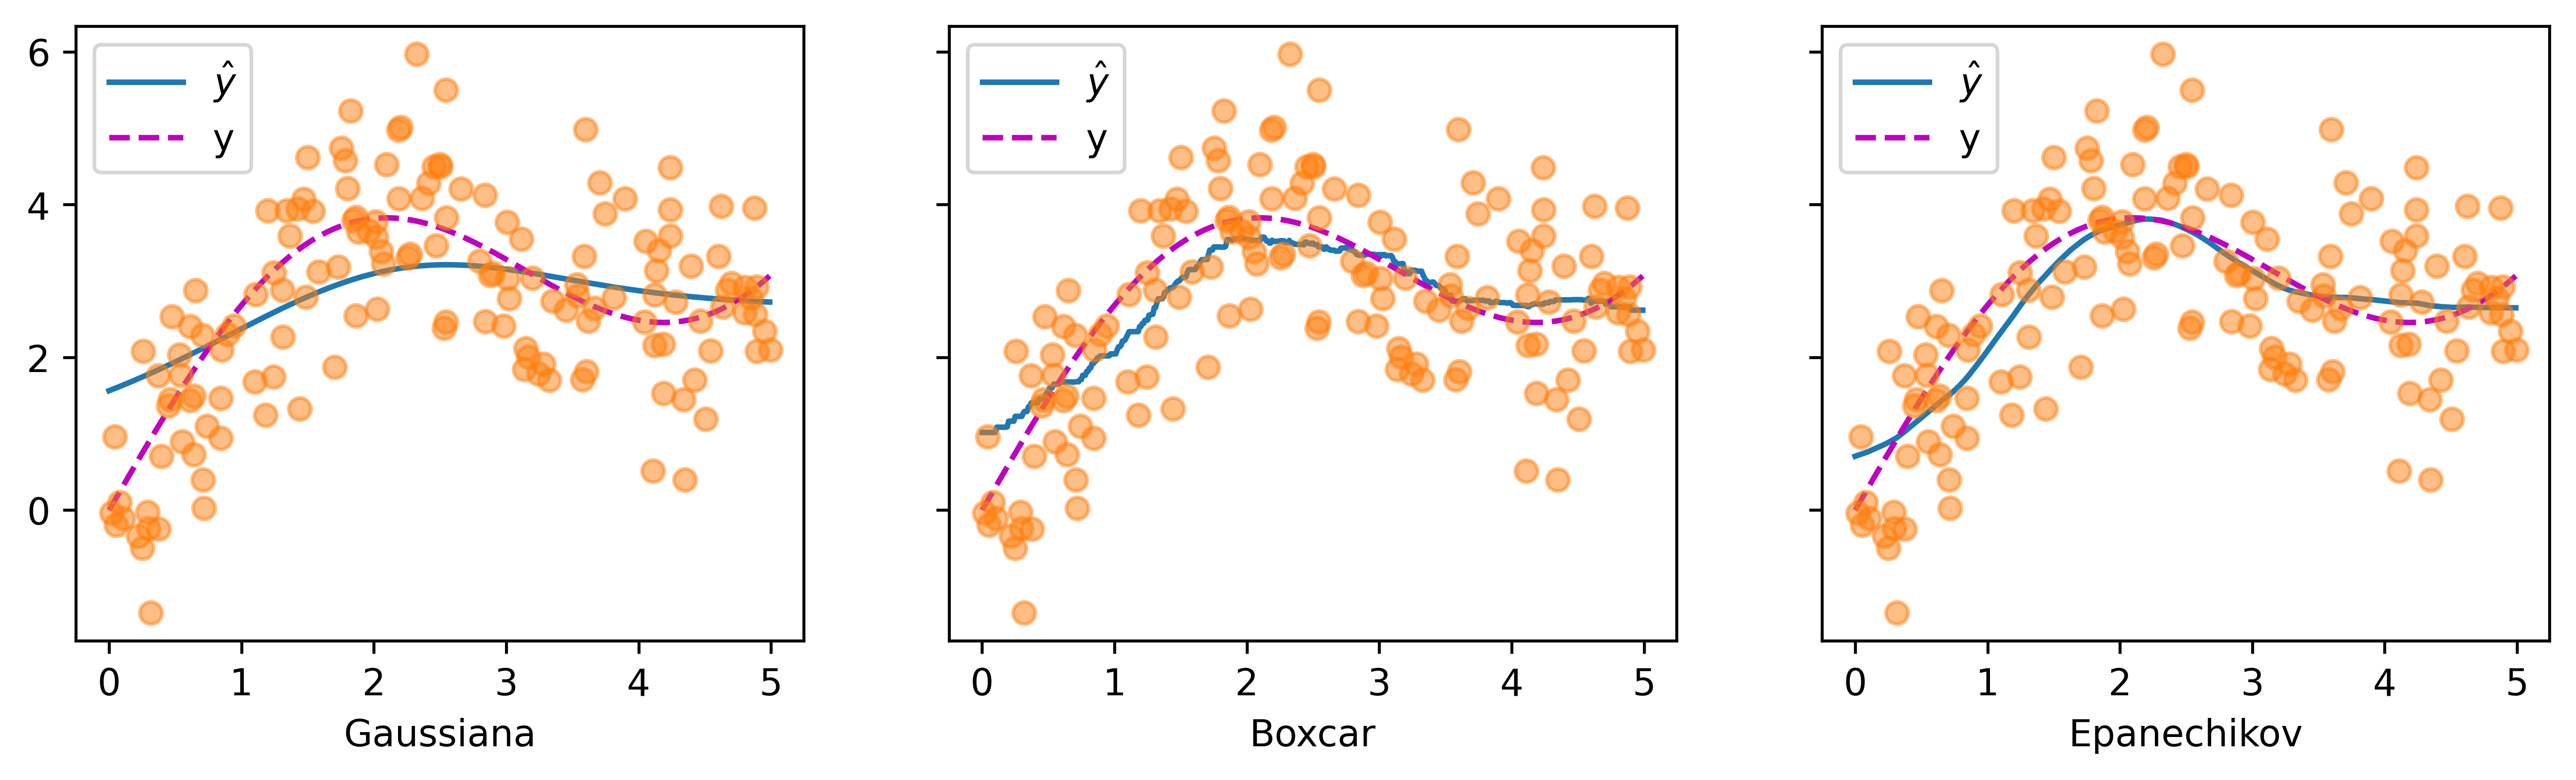
\includegraphics[width=\textwidth]{figures/chapter4/regression.png}
    \caption{Estimación de la función \( y \) mediante la estimación del valor de la variable objetivo sobre una partición equiespaciada del intervalo \( [0, 5] \) usando tres kérneles de similitud distintos.}
    \label{fig:regression}
\end{figure}

Esta forma de utilizar la atención es una forma de \textit{estimación de densidad de kernel}, una técnica clásica de inferencia no paramétrica que tiene la ventaja de que no requiere de ningún entrenamiento. Existen diversas heurísticas para elegir el \textit{kernel} \cite{silverman1986density} y puede probarse que si la anchura del \textit{kernel} se ajusta adecuadamente conforme se añaden observaciones entonces el método converge al valor real \( \E \llbracket y | x = x \rrbracket \) \cite{mack1982weak}.

\begin{figure}[tb]
    \centering
    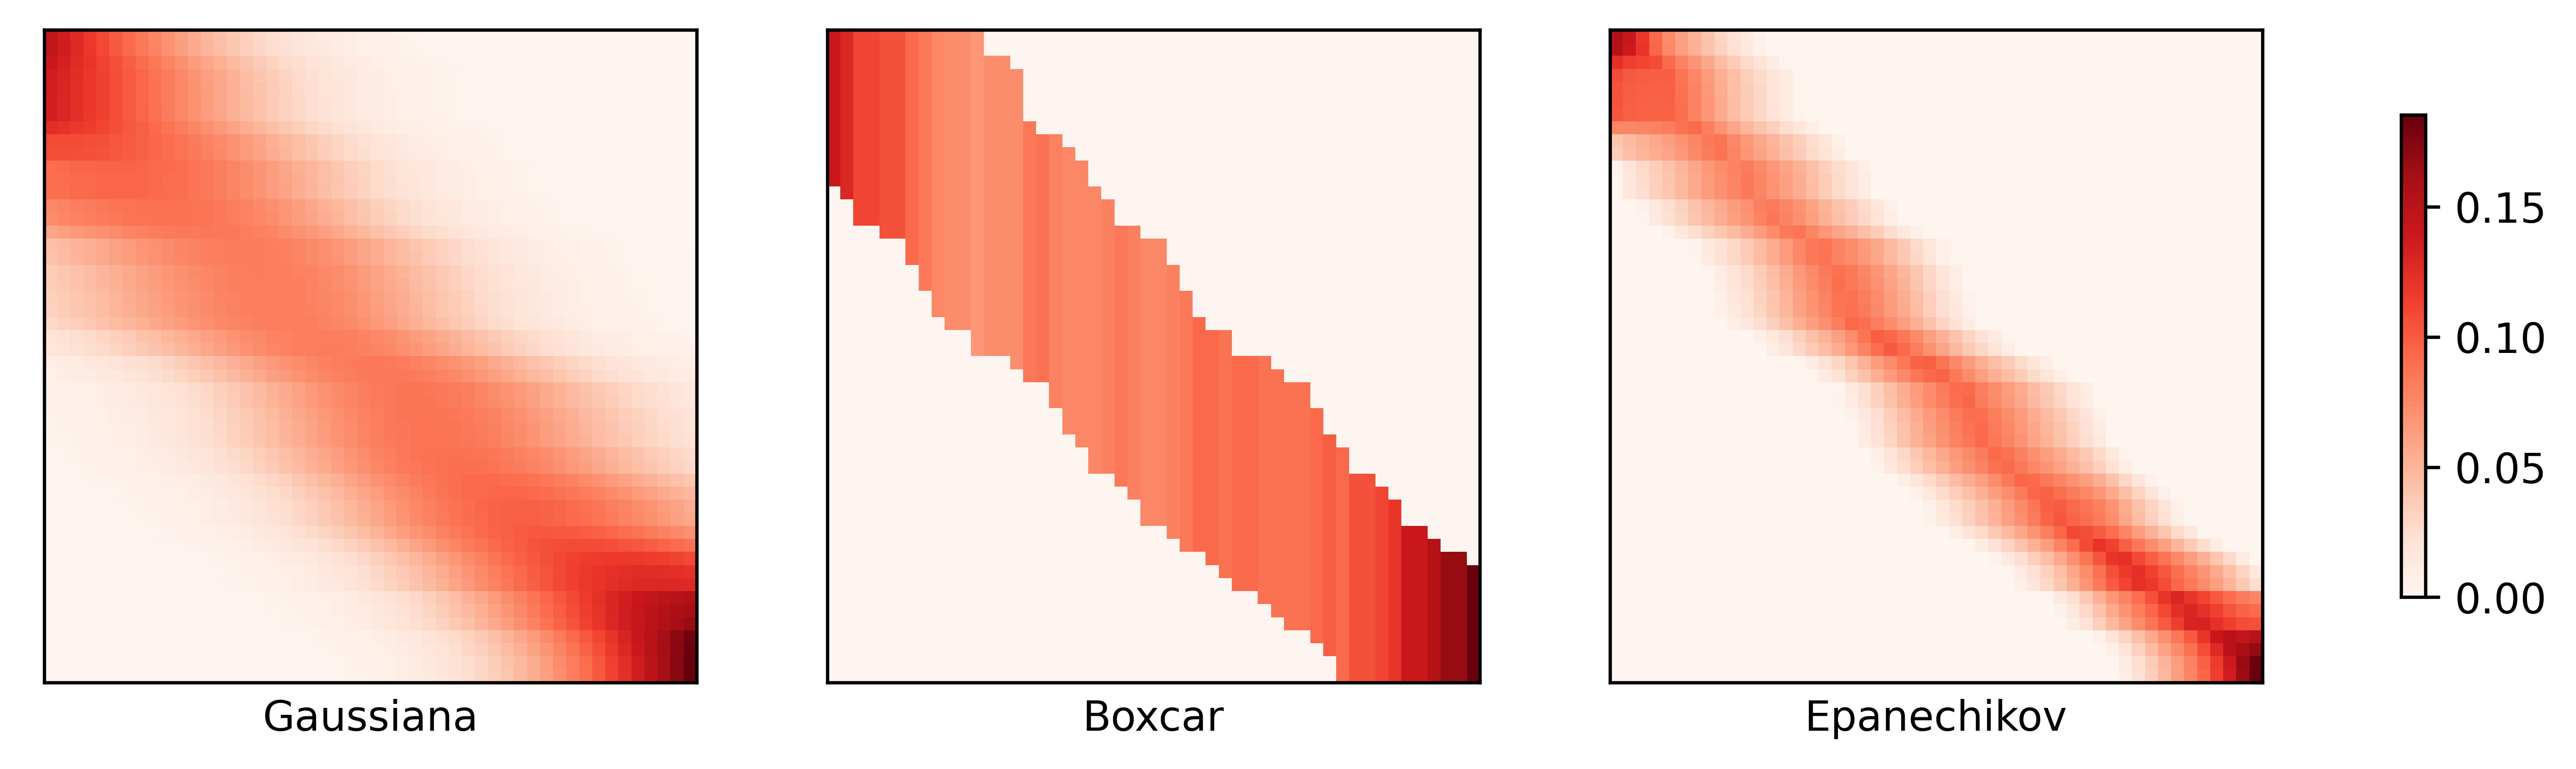
\includegraphics[width=\textwidth]{figures/chapter4/kernel.png}
    \caption{Visualización de los pesos de atención. Cada fila representa uno de los puntos aproximados y cada columna una componente del vector de atención. El color representa la magnitud de la componente.}
    \label{fig:kernel}
\end{figure}

El estudio del estimador de Nadaraya-Watson cumple un triple propósito: en primer lugar, muestra la flexibilidad de los métodos de atención y su relación con métodos clásicos de inferencia estadística. En segundo lugar, sirve para exhibir una de los grandes atributos de los métodos de atención: la posibilidad de visualizar los pesos de atención a fin de poder entender el funcionamiento del modelo. En tercer lugar, muestra lo decisivo de realizar una buena elección de la representación de la base de datos (claves y valores). En última instancia, la complejidad de elegir representaciones adecuadas lleva a diseñar esta representación de forma que sea \textit{aprendida} como una parte más de los parámetros del modelo.


\end{document}
